% =============================================================================
%  CHƯƠNG 2 – MÔ HÌNH HỆ THỐNG VÀ BÀI TOÁN TỐI ƯU
% =============================================================================
\chapter{MÔ HÌNH HỆ THỐNG VÀ BÀI TOÁN TỐI ƯU}
\label{ch:chuong2}

Chương này trình bày chi tiết mô hình hệ thống STAR-RIS hỗ trợ RSMA được
xem xét trong Luận văn, các giả thiết cơ bản, mô hình kênh truyền, mô
hình tín hiệu, tính toán SINR và tốc độ, phát biểu bài toán tối ưu (P0)
và cuối cùng là ánh xạ bài toán P0 sang quá trình ra quyết định Markov
(MDP) để áp dụng MADDPG ở Chương 3.

% -----------------------------------------------------------------------------
\section{Cấu hình hệ thống}
\label{sec:cau_hinh}

\subsection{Mô hình hệ thống và các giả thiết}

Hệ thống được xét bao gồm: một trạm gốc (BS) với $M=1$ anten (cấu hình
SISO), một STAR-RIS với $N=32$ phần tử thụ động hoạt động ở chế độ chia
sẻ năng lượng (ES), và $K=4$ thiết bị người dùng (UE) được phân thành hai
nhóm: $K_R=3$ người dùng trong vùng phản xạ R và $K_T=1$ người dùng
trong vùng truyền qua T \cite{liu2021starris}, \cite{mu2022simultaneously}, \cite{soleymani2024starris}. Hình \ref{fig:h2_1} minh họa cấu hình hệ thống, trong đó BS đặt cố định một phía của STAR-RIS, các UE phân bố ở cả hai vùng R và T. Người dùng vùng T chịu suy hao chướng ngại $-25$ dB trên đường truyền trực tiếp, mô phỏng kịch bản NLoS điển hình nơi STAR-RIS thực sự cần thiết để cung cấp kết nối tin cậy.

\begin{figure}[t]
  \centering
  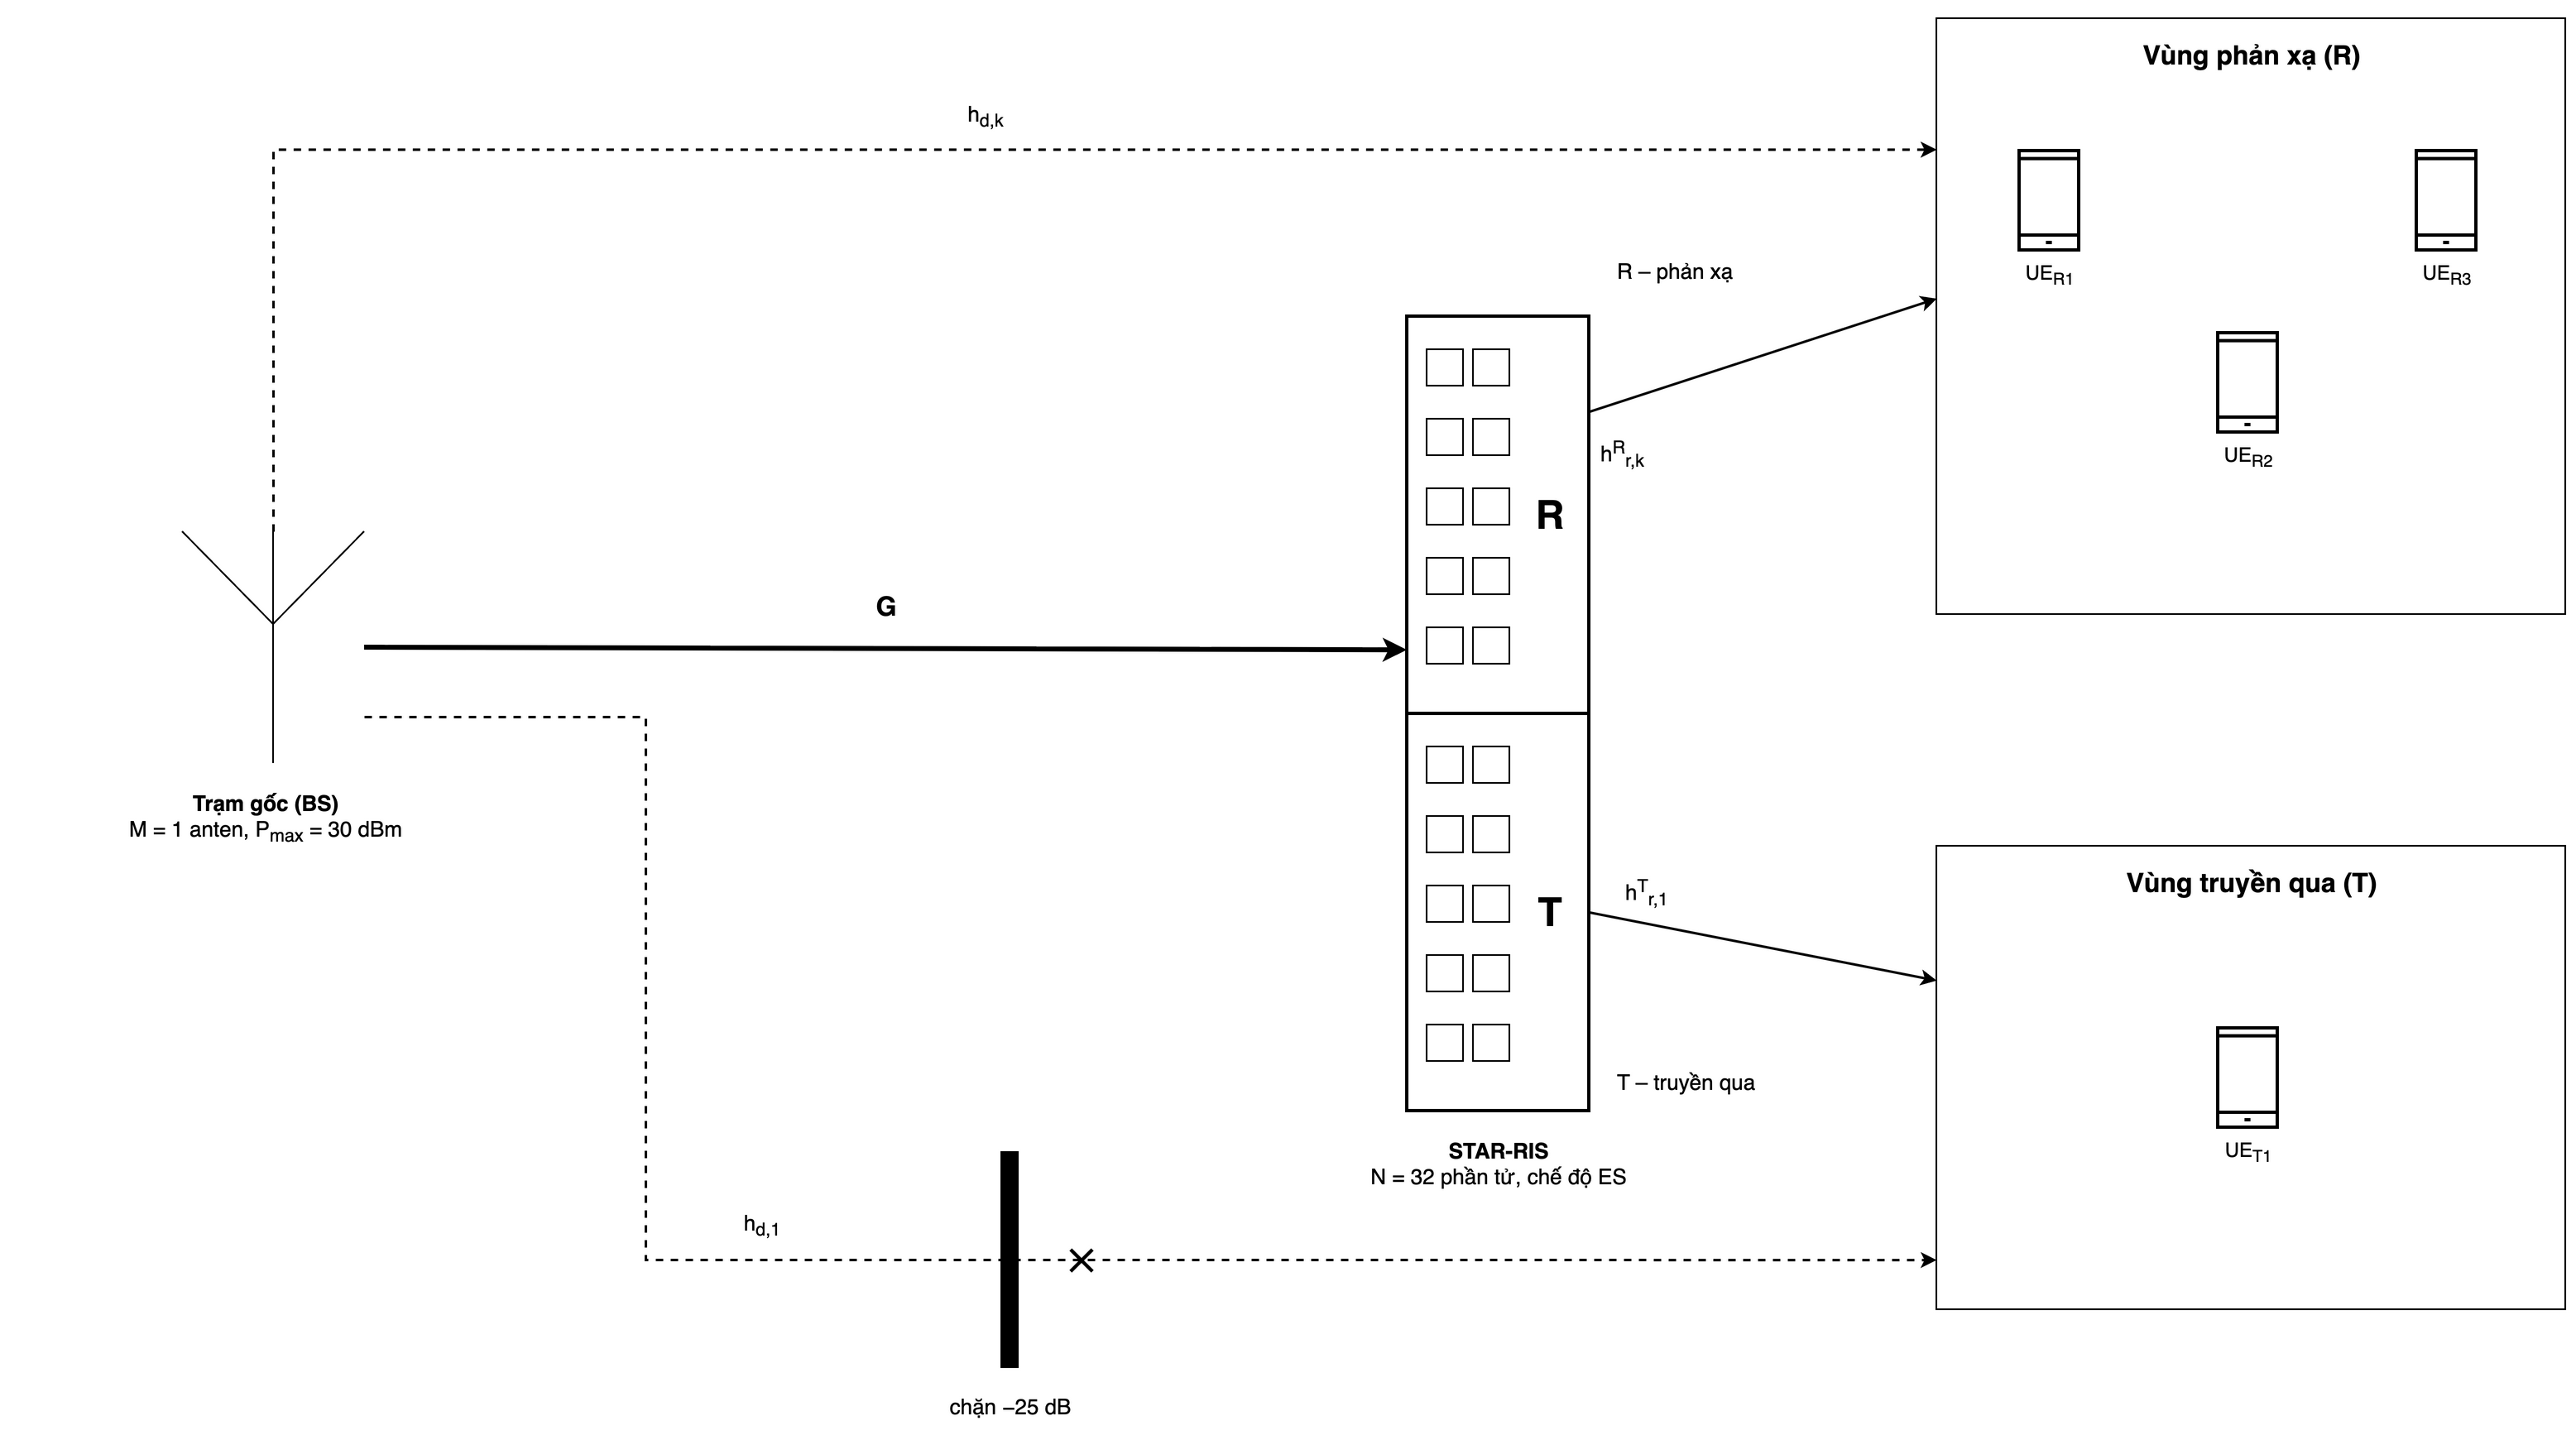
\includegraphics[width=0.96\linewidth]{figures/h2_1_cau_hinh_he_thong.png}
  \caption{Cấu hình hệ thống STAR-RIS hỗ trợ RSMA: BS đơn anten truyền tới
  $K=4$ người dùng qua STAR-RIS với $N=32$ phần tử (vùng R có 3 UE, vùng T
  có 1 UE chịu suy hao chướng ngại $-25$ dB).}
  \label{fig:h2_1}
\end{figure}

Các giả thiết chính của hệ thống:
\begin{enumerate}[label=(G\arabic*),leftmargin=*]
\item Trạm gốc nắm được thông tin trạng thái kênh hoàn hảo (perfect CSI)
của tất cả các kênh BS-UE, BS-RIS và RIS-UE.
\item Kênh truyền theo mô hình pha-đinh khối động (dynamic block fading):
\textbf{mỗi bước điều khiển $t$ tương ứng một khối coherence của kênh},
và thành phần pha-đinh phạm vi hẹp tiến hóa theo quá trình
Gauss--Markov bậc nhất
\begin{equation}
\tilde{h}_{t+1} \;=\; \rho\,\tilde{h}_t \;+\; \sqrt{1-\rho^2}\,
\boldsymbol{\epsilon}_t, \qquad \boldsymbol{\epsilon}_t \sim
\mathcal{CN}(\mathbf{0}, \mathbf{I}),
\label{eq:gauss_markov}
\end{equation}
áp dụng đồng thời cho $h_{d,k}$, $\mathbf{G}$ và $\mathbf{h}_{r,k}^X$,
với hệ số tương quan thời gian $\rho = 0{,}95$. Thứ tự chuyển trạng
thái trong một bước: tác tử quan sát kênh $\tilde{h}_t$, chọn hành động
$a_t$, phần thưởng được tính trên chính $\tilde{h}_t$ (bao gồm chi phí
tái cấu hình so với hành động đã áp ở bước trước), \emph{sau đó} kênh
mới tiến hóa sang $\tilde{h}_{t+1}$ và xuất hiện trong quan sát kế
tiếp. Một episode gồm $T=50$ khối coherence; hình học người dùng và
suy hao phạm vi rộng giữ cố định trong một episode và được lấy mẫu lại
ở đầu episode. Nhờ động lực kênh và chi phí tái cấu hình, hành động tại
bước $t$ ảnh hưởng thực sự tới các bước sau, nên hệ số chiết khấu
$\gamma$ và Bellman target có ý nghĩa đầy đủ.
\item Suy hao đường truyền tuân theo mô hình log-distance với các hệ số
khác nhau cho từng đoạn kênh.
\item Người dùng vùng truyền qua T chịu chướng ngại bổ sung $-25$~dB
trên kênh trực tiếp BS$\to$UE$_T$ để mô phỏng trường hợp NLoS điển hình
nơi STAR-RIS thực sự cần thiết.
\item Người dùng có thể giải mã hoàn hảo (perfect SIC) cho luồng chung.
\end{enumerate}

\subsection{Vị trí hình học và các tham số chính}

Bảng \ref{tab:he_thong_param} liệt kê các tham số hệ thống chính được sử
dụng trong Luận văn, bao gồm cấu hình BS, STAR-RIS, người dùng và các
ngưỡng QoS, công suất. Phiên bản đầy đủ với toàn bộ tham số mô phỏng và
huấn luyện được trình bày trong Bảng \ref{tab:simulation_parameters} ở
Chương 4.

\begin{table}[t]
\centering
\caption{Các tham số chính của hệ thống.}
\label{tab:he_thong_param}
\begin{tabular}{p{6cm} l}
\toprule
\textbf{Tham số} & \textbf{Giá trị} \\
\midrule
Số anten BS                                   & $M=1$ \\
Số phần tử STAR-RIS                           & $N=32$ \\
Số người dùng tổng                            & $K=4$ \\
Số người dùng vùng phản xạ                    & $K_R=3$ \\
Số người dùng vùng truyền qua                 & $K_T=1$ \\
Công suất phát tối đa $P_{\max}$              & $30$ dBm \\
Công suất tạp âm $\sigma^2$                   & $-90$ dBm \\
Suy hao chướng ngại UE$_T$                    & $-25$ dB \\
Yêu cầu QoS tối thiểu $R_{\min}$              & $0{,}3$ b/s/Hz \\
\bottomrule
\end{tabular}
\end{table}

\subsection{Tổng hợp giả thiết hệ thống}
\label{sec:assumptions}

Để khung phân tích nhất quán và dễ kiểm chứng, các giả thiết của hệ
thống được tổng hợp một cách có hệ thống trong Bảng
\ref{tab:assumptions}. Mỗi giả thiết đi kèm với biện minh khoa học
ngắn gọn, làm rõ lý do được chấp nhận trong bối cảnh nghiên cứu. Các
giả thiết này phản ánh thực tiễn phổ biến trong cộng đồng nghiên cứu
RIS/RSMA và đặt ra phạm vi áp dụng rõ ràng cho các kết quả của Luận
văn, đồng thời định hướng cho các nghiên cứu mở rộng được nêu trong
Kết luận.

\begin{table}[t]
\centering
\small
\caption{Tổng hợp các giả thiết hệ thống và lý do biện minh.}
\label{tab:assumptions}
\begin{tabular}{p{5.5cm} p{9cm}}
\toprule
\textbf{Giả thiết} & \textbf{Biện minh khoa học} \\
\midrule
A1. Thông tin trạng thái kênh hoàn hảo (Perfect CSI) tại BS &
Giả thiết tiêu chuẩn trong cộng đồng RIS/RSMA để cô lập hiệu ứng thuật toán \cite{liu2021starris}, \cite{mao2022rsma}. Trường hợp CSI không hoàn hảo được nêu trong Hướng nghiên cứu tiếp theo. \\
\addlinespace
A2. Pha-đinh Rayleigh độc lập (i.i.d.\ Rayleigh fading) &
Mô hình chuẩn cho môi trường tán xạ phong phú không có thành phần LoS chiếm ưu thế; được dùng rộng rãi trong nghiên cứu STAR-RIS \cite{mu2022simultaneously}. \\
\addlinespace
A3. Truyền đường xuống một cell, một BS đơn anten (SISO) &
Tập trung phân tích hiệu ứng STAR-RIS và RSMA mà không bị làm phức tạp bởi beamforming MIMO; cung cấp baseline rõ ràng để mở rộng MIMO sau này. \\
\addlinespace
A4. STAR-RIS thụ động, không khuếch đại (passive) &
Phù hợp với phần cứng STAR-RIS hiện tại; chế độ ES được chọn vì là chế độ tổng quát nhất \cite{liu2021starris}. \\
\addlinespace
A5. Ngân sách công suất phát hữu hạn $P_{\max} = 30$ dBm &
Tương ứng với mức công suất BS thực tế trong các small cell hoặc indoor AP \cite{wu2020smart}. \\
\addlinespace
A6. Pha-đinh khối động (dynamic block-fading): mỗi bước là một khối coherence, pha-đinh phạm vi hẹp tiến hóa Gauss--Markov với $\rho=0{,}95$ &
Mỗi bước điều khiển tương ứng một khối coherence; kênh tiến hóa theo tương quan thời gian giữa các bước (phương trình \eqref{eq:gauss_markov}), khiến hành động ảnh hưởng tới các bước sau và làm cho hệ số chiết khấu $\gamma$ có ý nghĩa. Chế độ static-block (kênh cố định cả episode) chỉ giữ để tái lập kết quả cũ. \\
\addlinespace
A9. STAR-RIS lý tưởng: pha liên tục, pha R/T độc lập, không tổn hao chèn, không trễ tái cấu hình (ideal independent-phase ES) &
Giả thiết chuẩn để cô lập giới hạn thuật toán; các tác động phần cứng (lượng tử pha, pha ghép cặp, insertion loss) được nêu trong Hạn chế/Hướng nghiên cứu tiếp theo. \\
\addlinespace
A7. Khử nhiễu liên tiếp hoàn hảo (Perfect SIC) tại UE &
Giả thiết tiêu chuẩn trong văn liệu RSMA \cite{mao2022rsma}; lỗi SIC được khảo sát trong \cite{gomes2024performance}. \\
\addlinespace
A8. Người dùng vùng truyền qua T chịu suy hao chướng ngại $-25$ dB &
Mô phỏng kịch bản NLoS điển hình nơi STAR-RIS thực sự cần thiết để cung cấp kết nối tin cậy. \\
\bottomrule
\end{tabular}

\vspace{0.2em}
\hfill {\footnotesize\itshape Nguồn: Tác giả tổng hợp (2026)}
\end{table}


% -----------------------------------------------------------------------------
\section{Mô hình kênh truyền}
\label{sec:kenh}

\subsection{Các thành phần kênh truyền}

Trong hệ thống xét, có ba loại kênh truyền chính được biểu diễn trong
Hình \ref{fig:h2_2}: kênh trực tiếp $h_{d,k}$ từ BS đến từng UE, kênh
$\mathbf{G}$ từ BS đến STAR-RIS, và các kênh $\mathbf{h}_{r,k}^X$ từ
STAR-RIS đến UE trong từng vùng. Mỗi kênh được mô hình hóa bằng phân
phối Rayleigh kết hợp với suy hao đường truyền log-distance, với các số
mũ suy hao khác nhau cho từng loại kênh.

\begin{figure}[t]
  \centering
  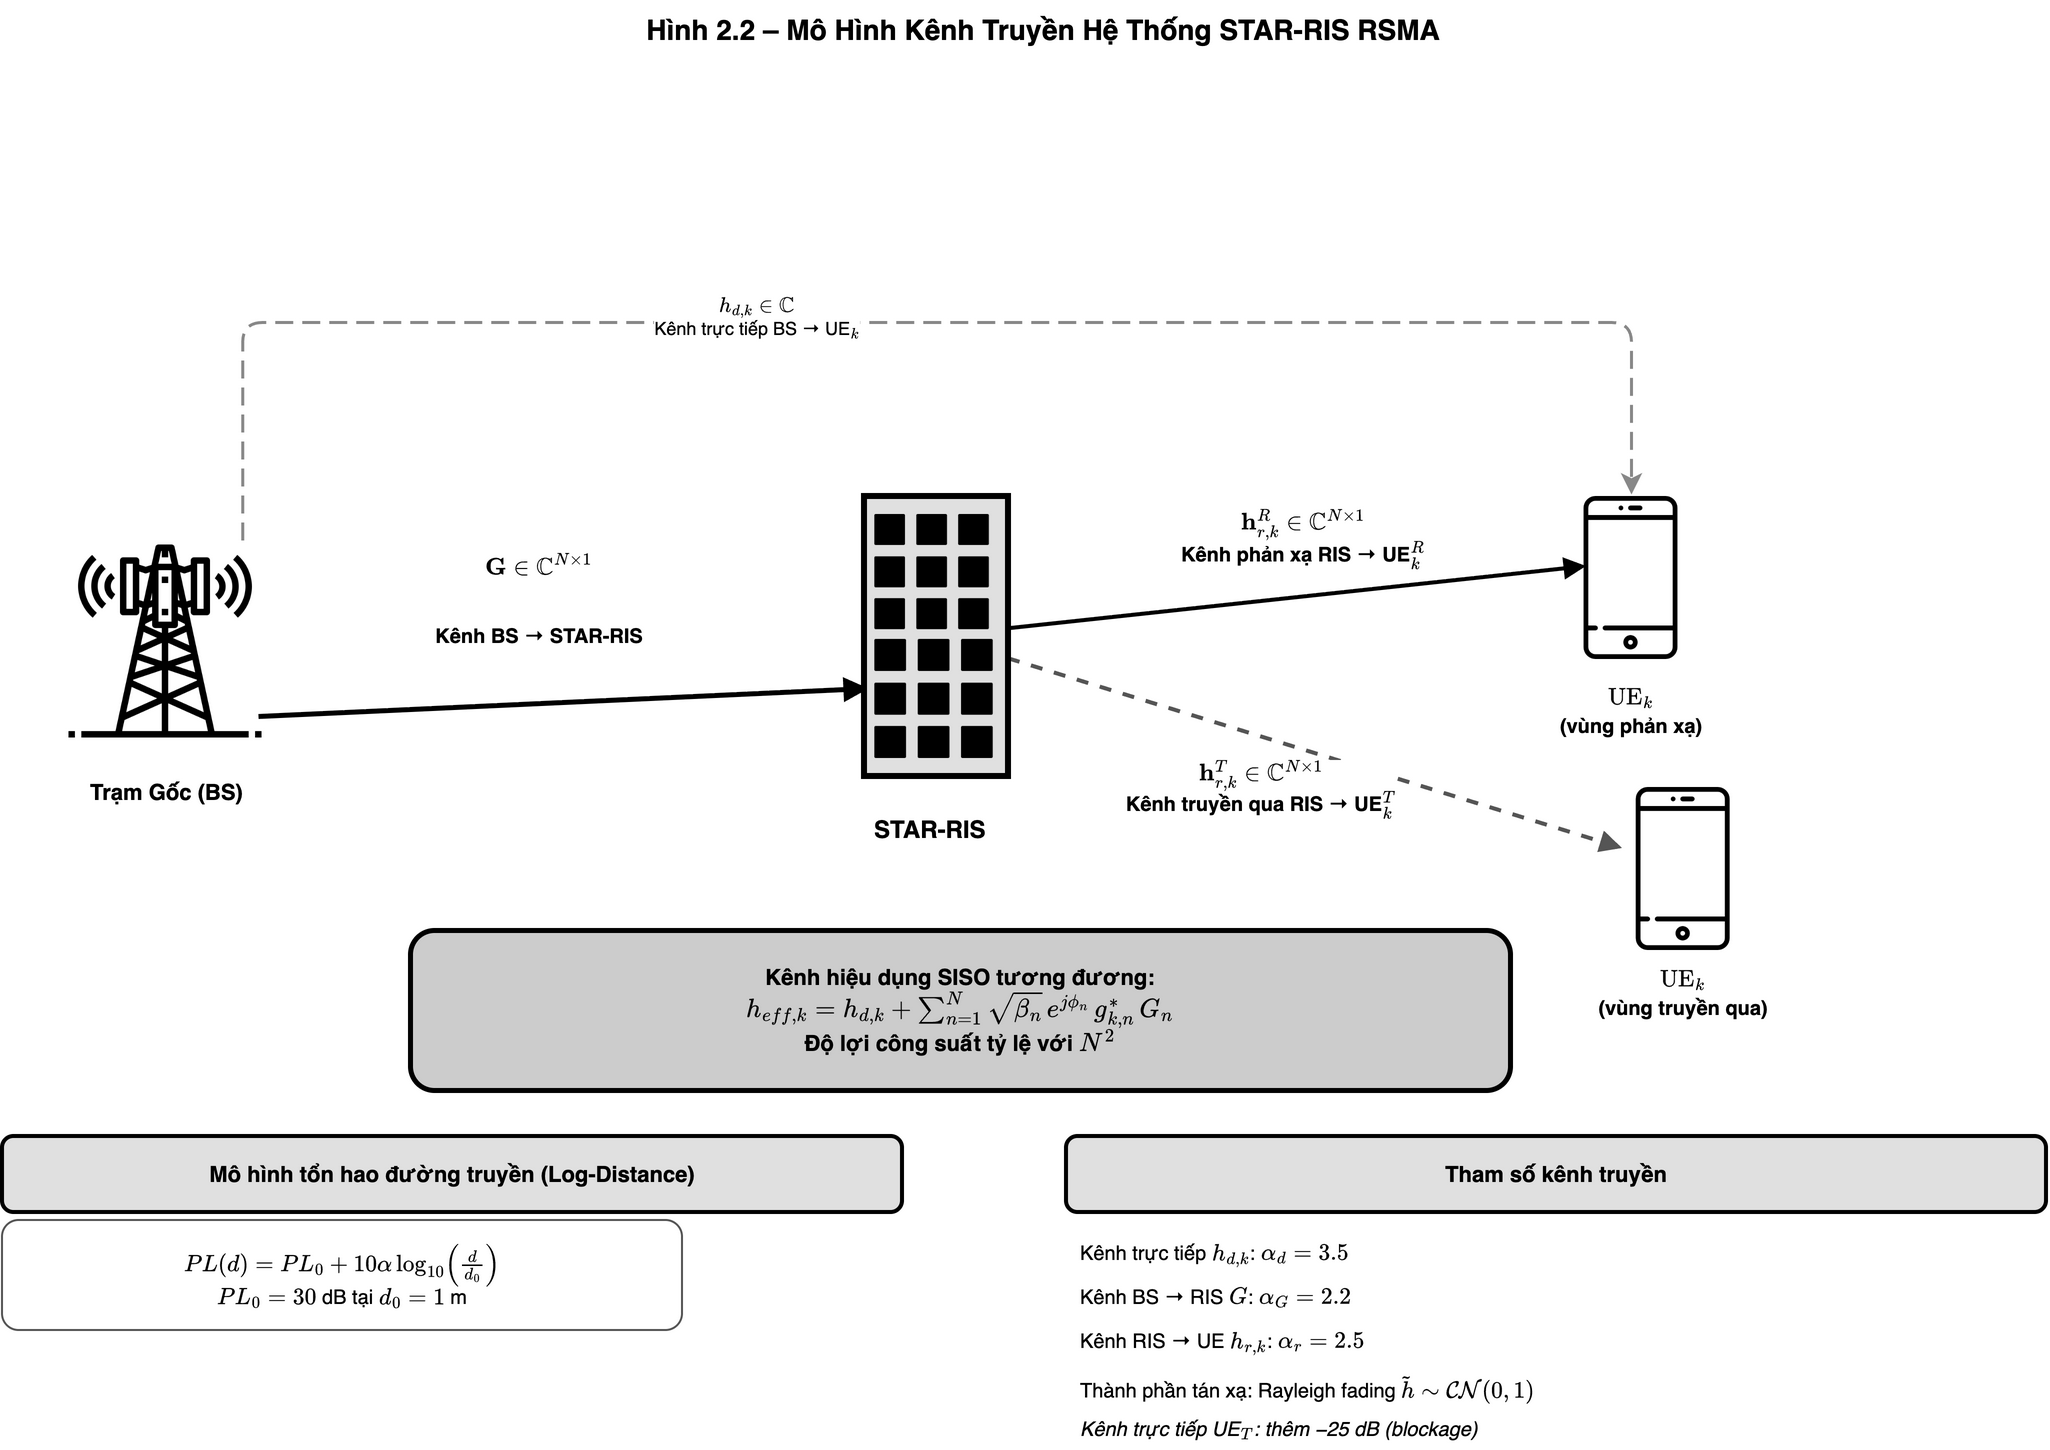
\includegraphics[width=0.96\linewidth]{figures/h2_2_kenh_truyen.png}
  \caption{Mô hình kênh truyền STAR-RIS RSMA: kênh trực tiếp $h_{d,k}$, kênh
  BS$\to$RIS $\mathbf{G}$, và kênh RIS$\to$UE $\mathbf{h}_{r,k}$ (cho cả hai
  vùng R và T).}
  \label{fig:h2_2}
\end{figure}

\textbf{Kênh trực tiếp BS$\to$UE$_k$:} ký hiệu $h_{d,k} \in \mathbb{C}$,
tuân theo phân phối Rayleigh $\mathcal{CN}(0, \zeta_{d,k}^2)$ với
$\zeta_{d,k}^2$ là độ lợi suy hao đường truyền tuyến trực tiếp.

\textbf{Kênh BS$\to$STAR-RIS:} ký hiệu $\mathbf{G} \in \mathbb{C}^{N \times 1}$,
mỗi phần tử là một biến phức Rayleigh độc lập.

\textbf{Kênh RIS$\to$UE$_k$:} ký hiệu $\mathbf{h}_{r,k}^X \in \mathbb{C}^{N \times 1}$
với $X \in \{R, T\}$ chỉ rõ vùng (phản xạ hay truyền qua).

\subsection{Mô hình suy hao đường truyền}

Suy hao đường truyền giữa hai điểm cách nhau $d$ mét tuân theo mô hình
log-distance \cite{wu2020smart}, \cite{mu2022simultaneously}:
\begin{equation}
  \mathrm{PL}(d) \;=\; \mathrm{PL}_0 + 10\,\alpha\,\log_{10}\!\frac{d}{d_0},
  \label{eq:pathloss}
\end{equation}
trong đó $\mathrm{PL}_0 = 30$ dB là suy hao tham chiếu tại $d_0=1$ m,
$\alpha$ là số mũ suy hao đường truyền. Các giá trị $\alpha$ khác nhau
cho từng loại kênh, được liệt kê trong Bảng \ref{tab:pathloss_param}.
Cụ thể, kênh trực tiếp BS$\to$UE có số mũ suy hao lớn nhất ($\alpha_d =
3{,}5$) phản ánh môi trường truyền sóng phức tạp, trong khi kênh
BS$\to$STAR-RIS được giả định gần đường truyền thẳng ($\alpha_G = 2{,}2$)
do thiết kế triển khai BS và RIS có tầm nhìn trực tiếp.

\begin{table}[t]
\centering
\caption{Số mũ suy hao đường truyền theo từng loại kênh.}
\label{tab:pathloss_param}
\begin{tabular}{p{6cm} c c}
\toprule
\textbf{Kênh} & \textbf{Ký hiệu} & \textbf{$\alpha$} \\
\midrule
Kênh trực tiếp BS$\to$UE                & $h_{d,k}$              & $3{,}5$ \\
Kênh BS$\to$STAR-RIS                    & $\mathbf{G}$           & $2{,}2$ \\
Kênh STAR-RIS$\to$UE                    & $\mathbf{h}_{r,k}$     & $2{,}5$ \\
\bottomrule
\end{tabular}
\end{table}

Kênh trực tiếp tới người dùng vùng T chịu thêm suy hao chướng ngại
$-25$ dB nhằm mô phỏng trường hợp NLoS, lý do STAR-RIS được triển khai.

\subsection{Hệ số phản xạ và truyền qua của STAR-RIS}
\label{sec:star_ris_coef}

Theo mục \ref{sec:starris} của Chương 1, mỗi phần tử thứ $n$ của
STAR-RIS có các hệ số phản xạ $\Phi_n^R$ và truyền qua $\Phi_n^T$ định
nghĩa trong \eqref{eq:starris_coef}.

\textbf{Quy ước về $\beta_n^X$:} Trong toàn bộ Luận văn này, đại lượng
$\beta_n^X \in [0,1]$ được định nghĩa là hệ số phân chia năng lượng
(power-splitting coefficient) tại phần tử $n$ trong vùng
$X \in \{R, T\}$, \textbf{không phải là biên độ}. Cụ thể:
\begin{equation}
|\Phi_n^X|^2 \;=\; \beta_n^X, \qquad
\Phi_n^X \;=\; \sqrt{\beta_n^X}\,e^{j\theta_n^X},
\label{eq:beta_def}
\end{equation}
nghĩa là $\sqrt{\beta_n^X}$ là biên độ phức của hệ số STAR-RIS, còn
$\beta_n^X$ là tỷ phần năng lượng tín hiệu được phân về vùng $X$. Với
quy ước này, định luật bảo toàn năng lượng STAR-RIS ở chế độ ES có
dạng tuyến tính theo $\beta$:
\begin{equation}
|\Phi_n^R|^2 + |\Phi_n^T|^2 \;=\; \beta_n^R + \beta_n^T \;=\; 1,
\quad \forall n \in \{1,\ldots,N\}.
\label{eq:es_constraint_full}
\end{equation}
Đây là dạng được sử dụng phổ biến trong các công trình STAR-RIS
\cite{liu2021starris}, \cite{mu2022simultaneously}. Hai ma trận pha dịch tổng
thể là:
\begin{align}
  \boldsymbol{\Phi}_R &= \mathrm{diag}\!\big(\sqrt{\beta_1^R}\,e^{j\theta_1^R},\,
  \ldots,\, \sqrt{\beta_N^R}\,e^{j\theta_N^R}\big), \label{eq:Phi_R}\\
  \boldsymbol{\Phi}_T &= \mathrm{diag}\!\big(\sqrt{\beta_1^T}\,e^{j\theta_1^T},\,
  \ldots,\, \sqrt{\beta_N^T}\,e^{j\theta_N^T}\big). \label{eq:Phi_T}
\end{align}

\textbf{Liên hệ giữa lý thuyết và cài đặt mô phỏng:} trong khuôn khổ
MADDPG ở Chương \ref{ch:chuong3}, tác tử RIS-R xuất trực tiếp giá trị
$\beta_n^R \in [0,1]$ (qua biến đổi affine $\beta_n^R = 0{,}5(a_n + 1)$
từ đầu ra $\tanh$). Giá trị $\beta_n^T$ được suy ra theo
\eqref{eq:es_constraint_full} là $\beta_n^T = 1 - \beta_n^R$, đảm bảo
bảo toàn năng lượng tự động ở mọi bước. Đây là lý do tác giả
chọn quy ước $\beta$ là hệ số năng lượng (chứ không phải biên độ): cách
chọn này cho phép ràng buộc tuyến tính đơn giản, tránh phải thực thi
ràng buộc bậc hai $\sqrt{\beta_n^R}^2 + \sqrt{\beta_n^T}^2 = 1$ phức tạp
hơn cho mạng nơ-ron.

\begin{figure}[t]
  \centering
  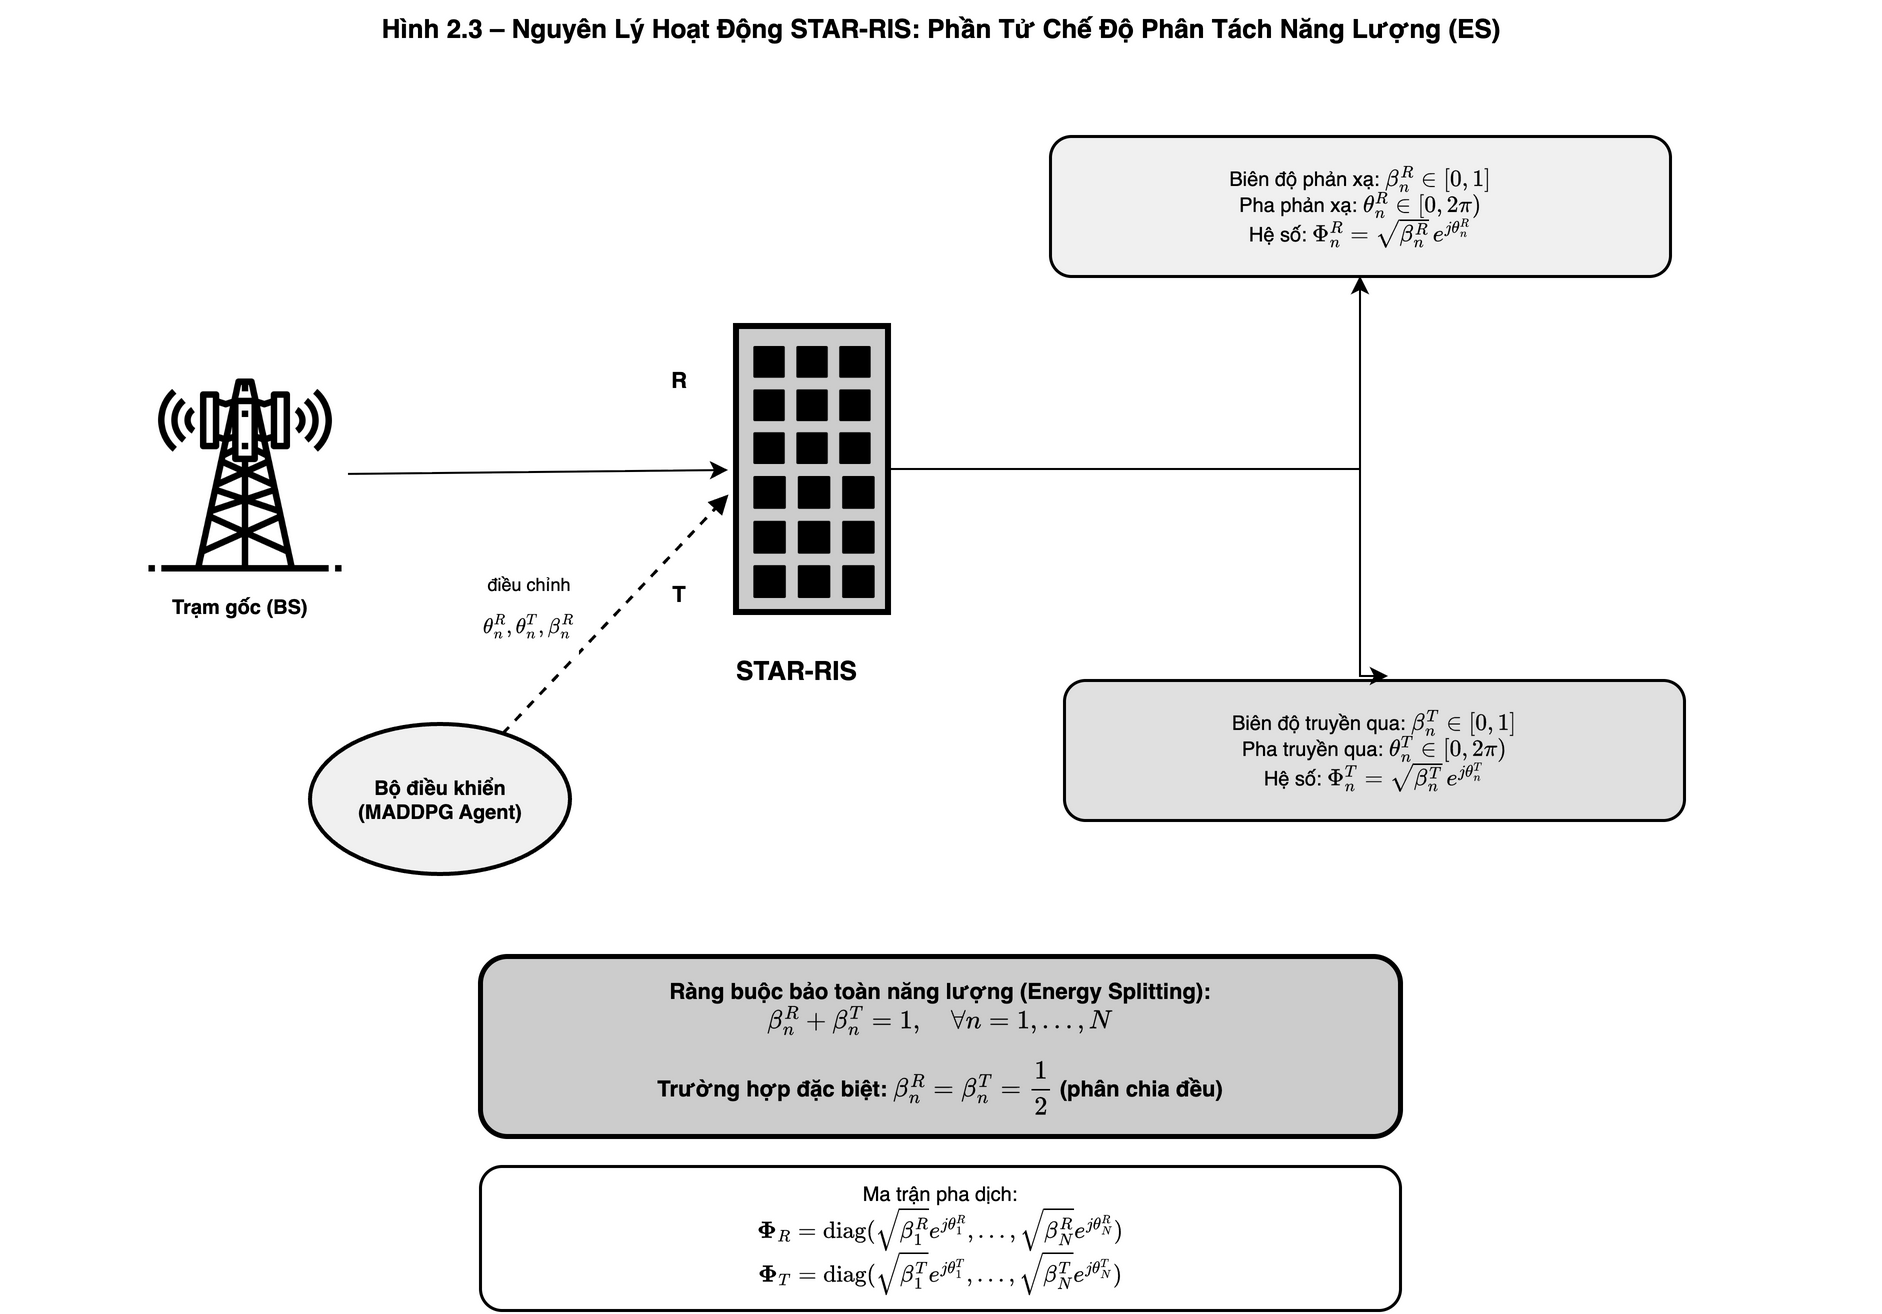
\includegraphics[width=0.92\linewidth]{figures/h2_3_star_ris_es.png}
  \caption{Nguyên lý hoạt động của phần tử STAR-RIS ở chế độ ES: sóng tới
  được phân tách thành sóng phản xạ (hệ số năng lượng $\beta_n^R$, pha
  $\theta_n^R$) và sóng truyền qua ($\beta_n^T$, $\theta_n^T$), thỏa
  $\beta_n^R + \beta_n^T = 1$.}
  \label{fig:h2_3}
\end{figure}

\subsection{Kênh hiệu dụng SISO tương đương}

Bằng cách gộp đường trực tiếp và đường gián tiếp qua STAR-RIS, ta thu
được kênh hiệu dụng SISO tương đương giữa BS và người dùng $k$
\cite{mao2022rsma}, \cite{hua2023learning}:
\begin{equation}
  h_{\text{eff},k} \;=\; h_{d,k} + \big(\mathbf{h}_{r,k}^X\big)^{\!H}\,
  \boldsymbol{\Phi}_X\,\mathbf{G}, \quad X \in \{R, T\},
  \label{eq:heff}
\end{equation}
hay tương đương dưới dạng tổng phần tử:
\begin{equation}
  h_{\text{eff},k} \;=\; h_{d,k} + \sum_{n=1}^{N} \sqrt{\beta_n^X}\,
  e^{j\theta_n^X}\, \big(\mathbf{h}_{r,k}^X\big)_n^*\,(\mathbf{G})_n.
  \label{eq:heff_sum}
\end{equation}
Hệ thức \eqref{eq:heff_sum} cho thấy rõ vai trò của STAR-RIS: bằng việc
chọn $\theta_n^X$ thích hợp, các pha của thành phần
$(\mathbf{h}_{r,k}^X)_n^*(\mathbf{G})_n$ có thể được căn chỉnh đồng
pha với $h_{d,k}$ để tối đa $|h_{\text{eff},k}|^2$. Khi $\theta_n^X$ được
chọn lý tưởng, độ lợi công suất kênh hiệu dụng tỷ lệ với $N^2$, nghĩa là
gấp đôi số phần tử RIS sẽ làm tăng độ lợi gấp bốn, một trong
những lý do khiến RIS được coi là công nghệ then chốt cho 6G.

% -----------------------------------------------------------------------------
\section{Mô hình tín hiệu RSMA, SINR và tốc độ đạt được}
\label{sec:rsma_signal}

\subsection{Tín hiệu phát và tín hiệu thu}

Theo công thức \eqref{eq:rsma_signal}, tín hiệu phát hợp nhất tại BS là
$x = \sqrt{P_c}\,s_c + \sum_{k=1}^{K}\sqrt{P_k}\,s_k$. Tín hiệu thu tại
người dùng $k$ qua kênh hiệu dụng là:
\begin{equation}
  y_k \;=\; h_{\text{eff},k}\,x + n_k
        \;=\; h_{\text{eff},k}\Big(\sqrt{P_c}\,s_c + \sum_{j=1}^{K}\sqrt{P_j}\,s_j\Big)
        + n_k,
  \label{eq:yk}
\end{equation}
với $n_k \sim \mathcal{CN}(0, \sigma^2)$ là tạp âm Gauss phức.

\subsection{Giải mã luồng chung và SINR luồng chung}

Người dùng $k$ trước tiên giải mã luồng chung $s_c$ trong khi xem các
luồng riêng (kể cả luồng riêng của chính mình) là nhiễu. SINR của luồng
chung tại UE $k$ là:
\begin{equation}
  \gamma_{c,k} \;=\; \frac{P_c\,|h_{\text{eff},k}|^2}
                          {\sum_{j=1}^{K} P_j\,|h_{\text{eff},k}|^2 + \sigma^2}.
  \label{eq:sinr_c}
\end{equation}
Tốc độ luồng chung mà UE $k$ có thể giải mã thành công là
$R_{c,k} = \log_2(1+\gamma_{c,k})$. Như đã giải thích trong Chương 1, vì
luồng chung phải được mọi người dùng giải mã, tốc độ luồng chung
khả thi bị giới hạn theo công thức $R_c = \min_k R_{c,k}$
\eqref{eq:rc_minmax}.

\subsection{Áp dụng SIC và SINR luồng riêng}

Sau khi giải mã thành công $\hat s_c$, UE $k$ trừ ảnh hưởng của nó khỏi
tín hiệu thu để có tín hiệu còn lại. SINR của luồng riêng của UE $k$
khi đó là:
\begin{equation}
  \gamma_{p,k} \;=\; \frac{P_k\,|h_{\text{eff},k}|^2}
                          {\sum_{j=1,\,j\neq k}^{K} P_j\,|h_{\text{eff},k}|^2 + \sigma^2}.
  \label{eq:sinr_p}
\end{equation}
Tốc độ luồng riêng là $R_{p,k} = \log_2(1+\gamma_{p,k})$.

\subsection{Tốc độ người dùng và tổng tốc độ hệ thống}

Theo định nghĩa của RSMA \cite{mao2022rsma}, tốc độ tổng mà UE $k$
nhận được là $R_k = c_k\,R_c + R_{p,k}$ \eqref{eq:rk}, và tổng tốc độ
toàn hệ thống là:
\begin{equation}
  R_{\text{sum}} \;=\; \sum_{k=1}^{K} R_k
                  \;=\; R_c + \sum_{k=1}^{K} R_{p,k},
  \label{eq:rsum}
\end{equation}
do $\sum_k c_k = 1$.

% -----------------------------------------------------------------------------
\section{Bài toán tối ưu (P0)}
\label{sec:P0}

\subsection{Phát biểu bài toán}

Mục tiêu của hệ thống là tối đa hóa tổng tốc độ $R_{\text{sum}}$ bằng
cách lựa chọn đồng thời ba nhóm biến tối ưu (xem Hình \ref{fig:h2_4}):
\begin{itemize}[leftmargin=*]
\item Vector công suất $\mathbf{P} = (P_c, P_1, P_2, \ldots, P_K)$;
\item Vector pha và biên độ STAR-RIS
$\boldsymbol{\Theta} = (\{\theta_n^R, \theta_n^T, \beta_n^R\}_{n=1}^{N})$
(do $\beta_n^T = 1 - \beta_n^R$ từ ràng buộc bảo toàn năng lượng);
\item Vector tỷ lệ tách $\mathbf{C} = (c_1, c_2, \ldots, c_K)$.
\end{itemize}

Hình \ref{fig:h2_4} biểu diễn cấu trúc tổng thể của bài toán P0, bao
gồm hàm mục tiêu max $R_{\text{sum}}$, ba nhóm biến tối ưu và sáu nhóm
ràng buộc về công suất, năng lượng, tỷ lệ tách, pha, biên độ và QoS.
Phần dưới của hình tóm tắt tính phi lồi của bài toán và động lực sử
dụng MADDPG để giải.

\begin{figure}[t]
  \centering
  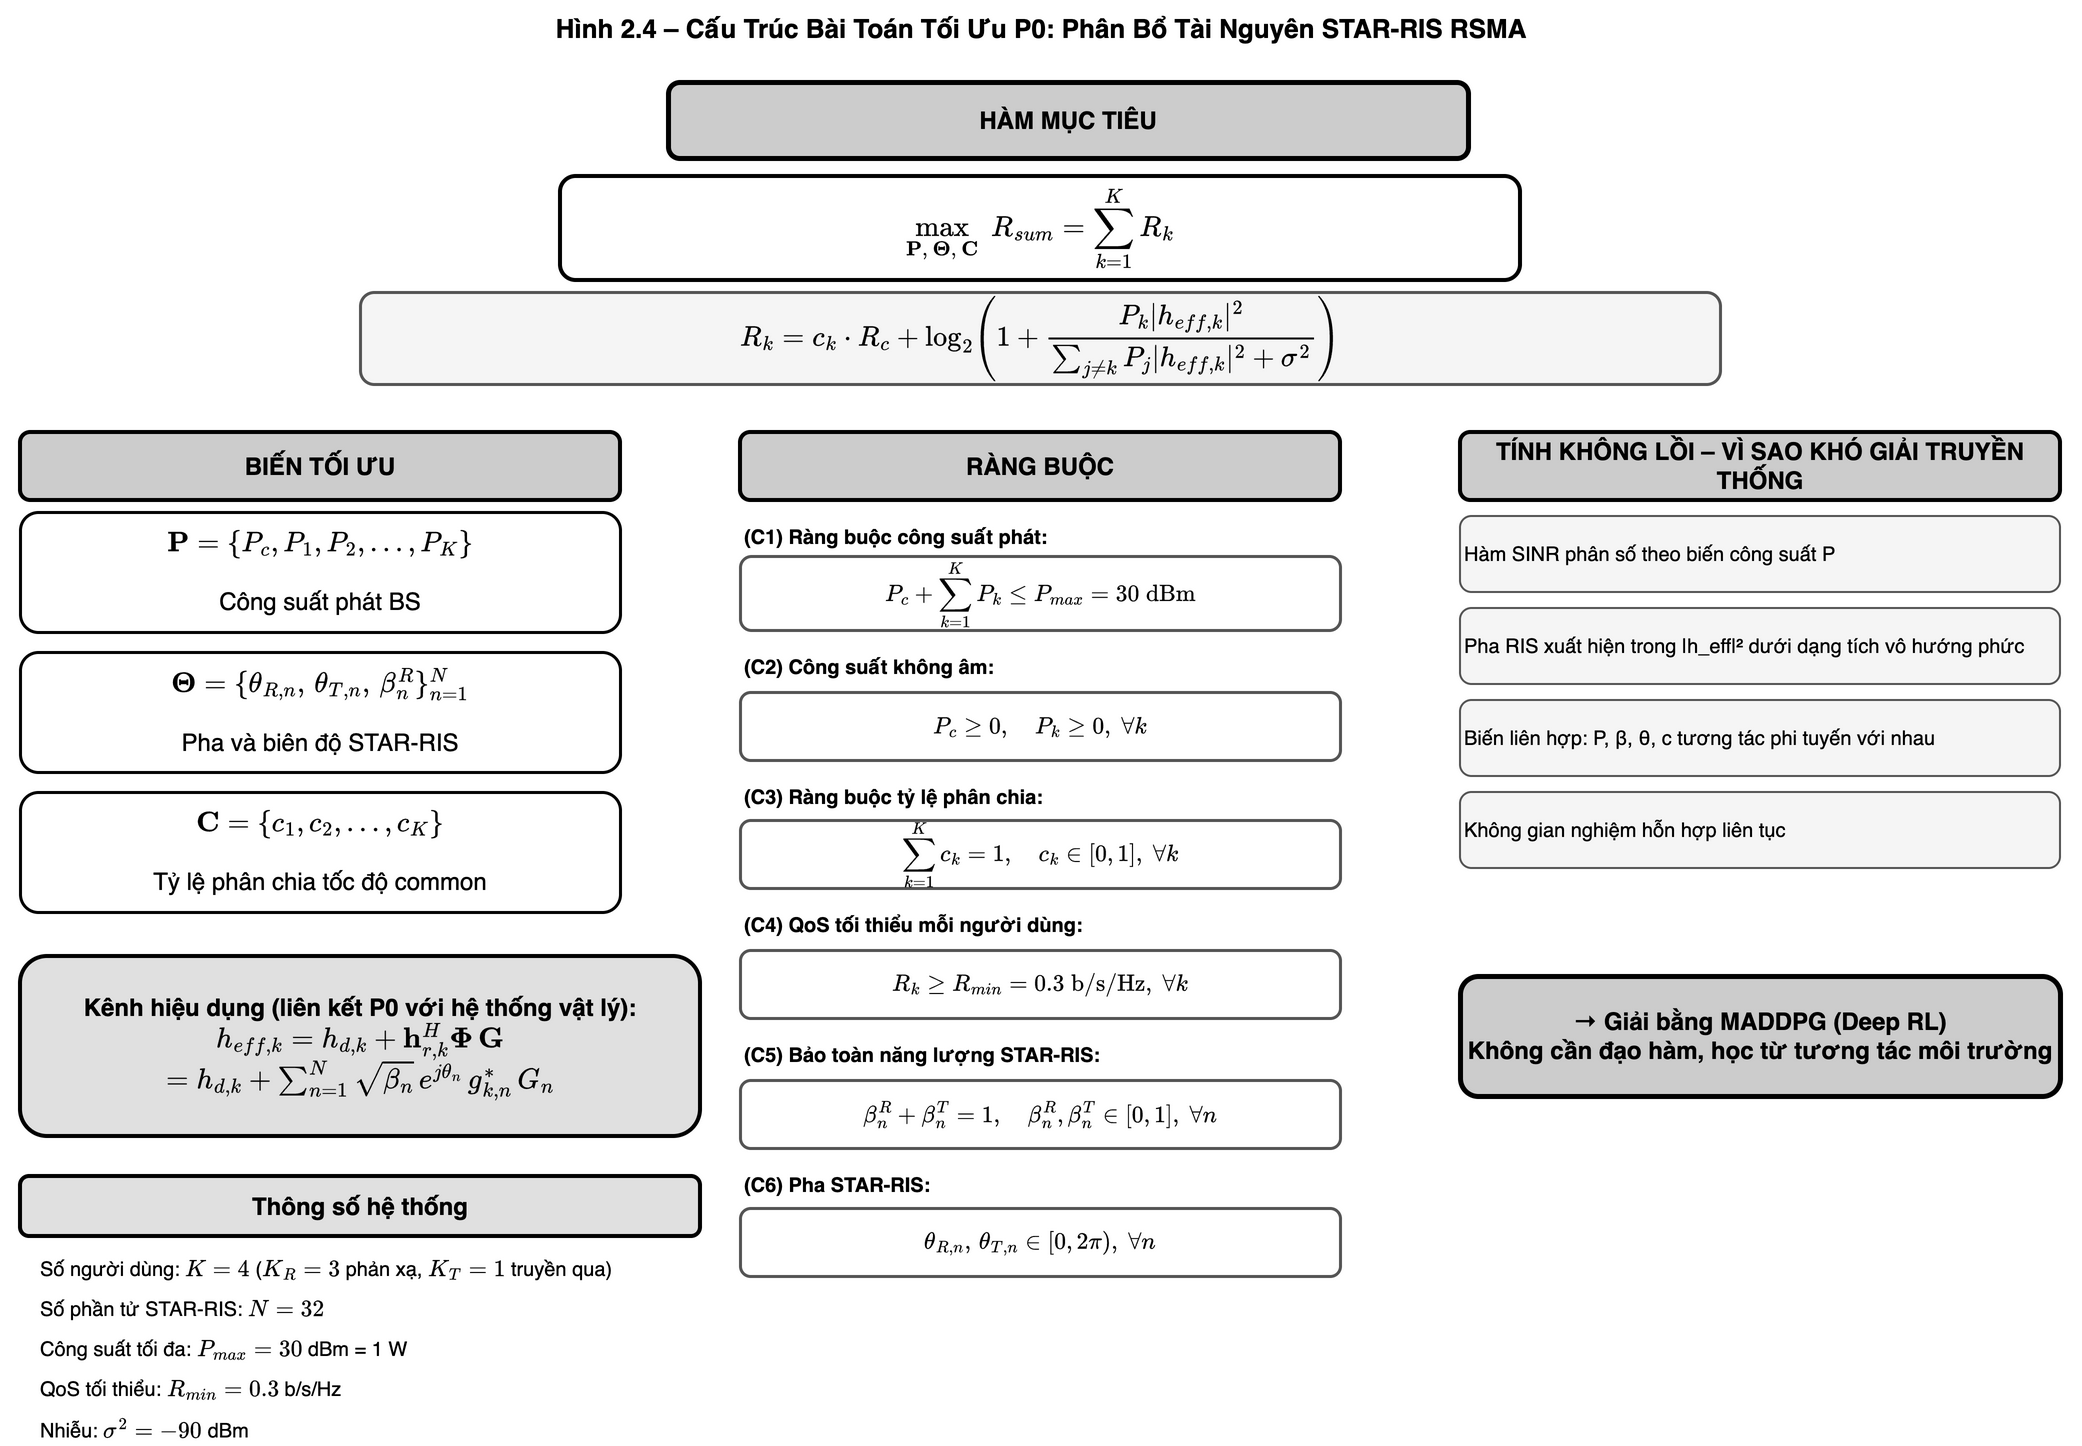
\includegraphics[width=0.95\linewidth]{figures/h2_4_bai_toan_p0.png}
  \caption{Cấu trúc bài toán tối ưu P0: hàm mục tiêu max $R_{\text{sum}}$,
  ba nhóm biến tối ưu và sáu nhóm ràng buộc.}
  \label{fig:h2_4}
\end{figure}

Bài toán tối ưu P0 được phát biểu như sau:

\begin{equation}
\begin{aligned}
(\text{P0}):\quad & \max_{\mathbf{P},\,\boldsymbol{\Theta},\,\mathbf{C}}
\; R_{\text{sum}} = \sum_{k=1}^{K} R_k \\[2pt]
\text{s.t.}\quad
& (\text{C1})\quad P_c + \sum_{k=1}^{K} P_k \;\leq\; P_{\max}, \\
& (\text{C2})\quad P_c \geq 0,\; P_k \geq 0,\; \forall k, \\
& (\text{C3})\quad \sum_{k=1}^{K} c_k = 1,\; c_k \in [0,1],\; \forall k, \\
& (\text{C4})\quad R_k \geq R_{\min},\; \forall k \in \{1,\ldots,K\}, \\
& (\text{C5})\quad \beta_n^R + \beta_n^T = 1,\;
                   \beta_n^R, \beta_n^T \in [0,1],\; \forall n, \\
& (\text{C6})\quad \theta_n^R, \theta_n^T \in [0, 2\pi),\; \forall n.
\end{aligned}
\label{eq:P0}
\end{equation}

Các ràng buộc có ý nghĩa: (C1)--(C2) đảm bảo công suất phát không vượt
$P_{\max}=30$~dBm; (C3) đảm bảo tổng tỷ lệ phân chia luồng chung bằng 1;
(C4) ràng buộc QoS yêu cầu mỗi UE đạt tốc độ tối thiểu
$R_{\min}=0{,}3$~b/s/Hz; (C5)--(C6) là các ràng buộc nội tại của STAR-RIS.

\textbf{Nhận xét quan trọng.} So với mô hình P0 cổ điển trong các nghiên
cứu trước \cite{mao2022rsma}, \cite{gomes2024performance}, bài toán P0 mà Luận
văn xem xét có hai điểm khác biệt: (i) ràng buộc QoS (C4) được thêm vào
một cách tường minh để phản ánh yêu cầu dịch vụ trong các kịch bản 6G
(khi giải bằng DRL, ràng buộc cứng này được xử lý qua một surrogate
ràng buộc mềm với cập nhật đối ngẫu, xem Mục \ref{sec:reward_surrogate});
và (ii) biên độ $\beta_n^R$ được xem là biến tối ưu thay
vì cố định ở giá trị $1/2$, qua đó cho phép phân phối năng lượng giữa hai
vùng linh hoạt hơn.

\subsection{Tính phi lồi và động lực sử dụng DRL}

Bài toán P0 \eqref{eq:P0} là một bài toán phi lồi rất khó giải vì nhiều
nguyên nhân kết hợp \cite{wu2020smart}, \cite{mao2022rsma}, \cite{irkicatal2024deep}:

\textbf{(i) Hàm SINR \eqref{eq:sinr_c} và \eqref{eq:sinr_p} là tỷ số phân
thức theo công suất.} Do đó hàm mục tiêu $R_{\text{sum}}$, là tổng các
$\log_2(1+\gamma)$, không lồi trên không gian công suất $\mathbf{P}$.

\textbf{(ii) Biến pha $\theta_n$ xuất hiện trong $h_{\text{eff},k}$ dưới
dạng hàm mũ phức $e^{j\theta_n}$.} Bình phương biên độ $|h_{\text{eff},k}|^2$
mở rộng thành tổng các tích chéo $\cos(\theta_n - \theta_m)$, không lồi
theo $\theta$.

\textbf{(iii) Tương tác phi tuyến giữa các nhóm biến.} $\mathbf{P}$,
$\boldsymbol{\Theta}$, $\mathbf{C}$ liên kết với nhau qua hàm mục tiêu và
ràng buộc QoS theo cách phi tuyến phức tạp.

\textbf{(iv) Ràng buộc QoS (C4) là phi lồi.} Tập khả thi $R_k \geq R_{\min}$
được định nghĩa qua các hàm $\log$ của tỷ số phi tuyến, không lồi.

Các phương pháp cổ điển (BCD, SDR, AO) tuy có thể tìm điểm dừng cục bộ
nhưng chi phí tính toán cao, không phù hợp cho cập nhật thời gian thực
trong các kịch bản 6G với kênh biến thiên ở mức ms. Hơn nữa, các phương
pháp này thường đòi hỏi hiểu biết chính xác về mô hình kênh, một giả
thiết không phải lúc nào cũng đúng trong thực tế. Vì vậy, Luận văn lựa
chọn hướng tiếp cận học tăng cường sâu để giải bài toán P0.

% -----------------------------------------------------------------------------
\section{Ánh xạ sang quá trình ra quyết định Markov}
\label{sec:mdp}

Để áp dụng DRL/MADDPG, bài toán P0 cần được ánh xạ sang một MDP với bộ năm
$(\mathcal{S}, \mathcal{A}, \mathcal{P}, \mathcal{R}, \gamma)$ phù hợp với
cơ chế ba tác tử chuyên dụng. Hình \ref{fig:h2_5} tóm lược ánh xạ MDP,
trong đó không gian trạng thái 550 chiều được phân thành ba phần tương
ứng quan sát cục bộ của từng tác tử, không gian hành động 105 chiều bao
gồm công suất, biên độ, pha và tỷ lệ tách, còn hàm phần thưởng là
Lagrangian surrogate giữa sum-rate và mức đáp ứng QoS. Bố cục chi tiết
của quan sát/hành động được sinh tự động từ mã nguồn qua
\texttt{observation\_schema()} / \texttt{action\_schema()}
(file \texttt{observation\_schema.json}), bảo đảm mô tả dưới đây khớp
tuyệt đối với cài đặt.

% LUU Y: hinh h2_5/h2_6 can ve lai theo so chieu moi (550/655) sau refactor.
\begin{figure}[t]
  \centering
  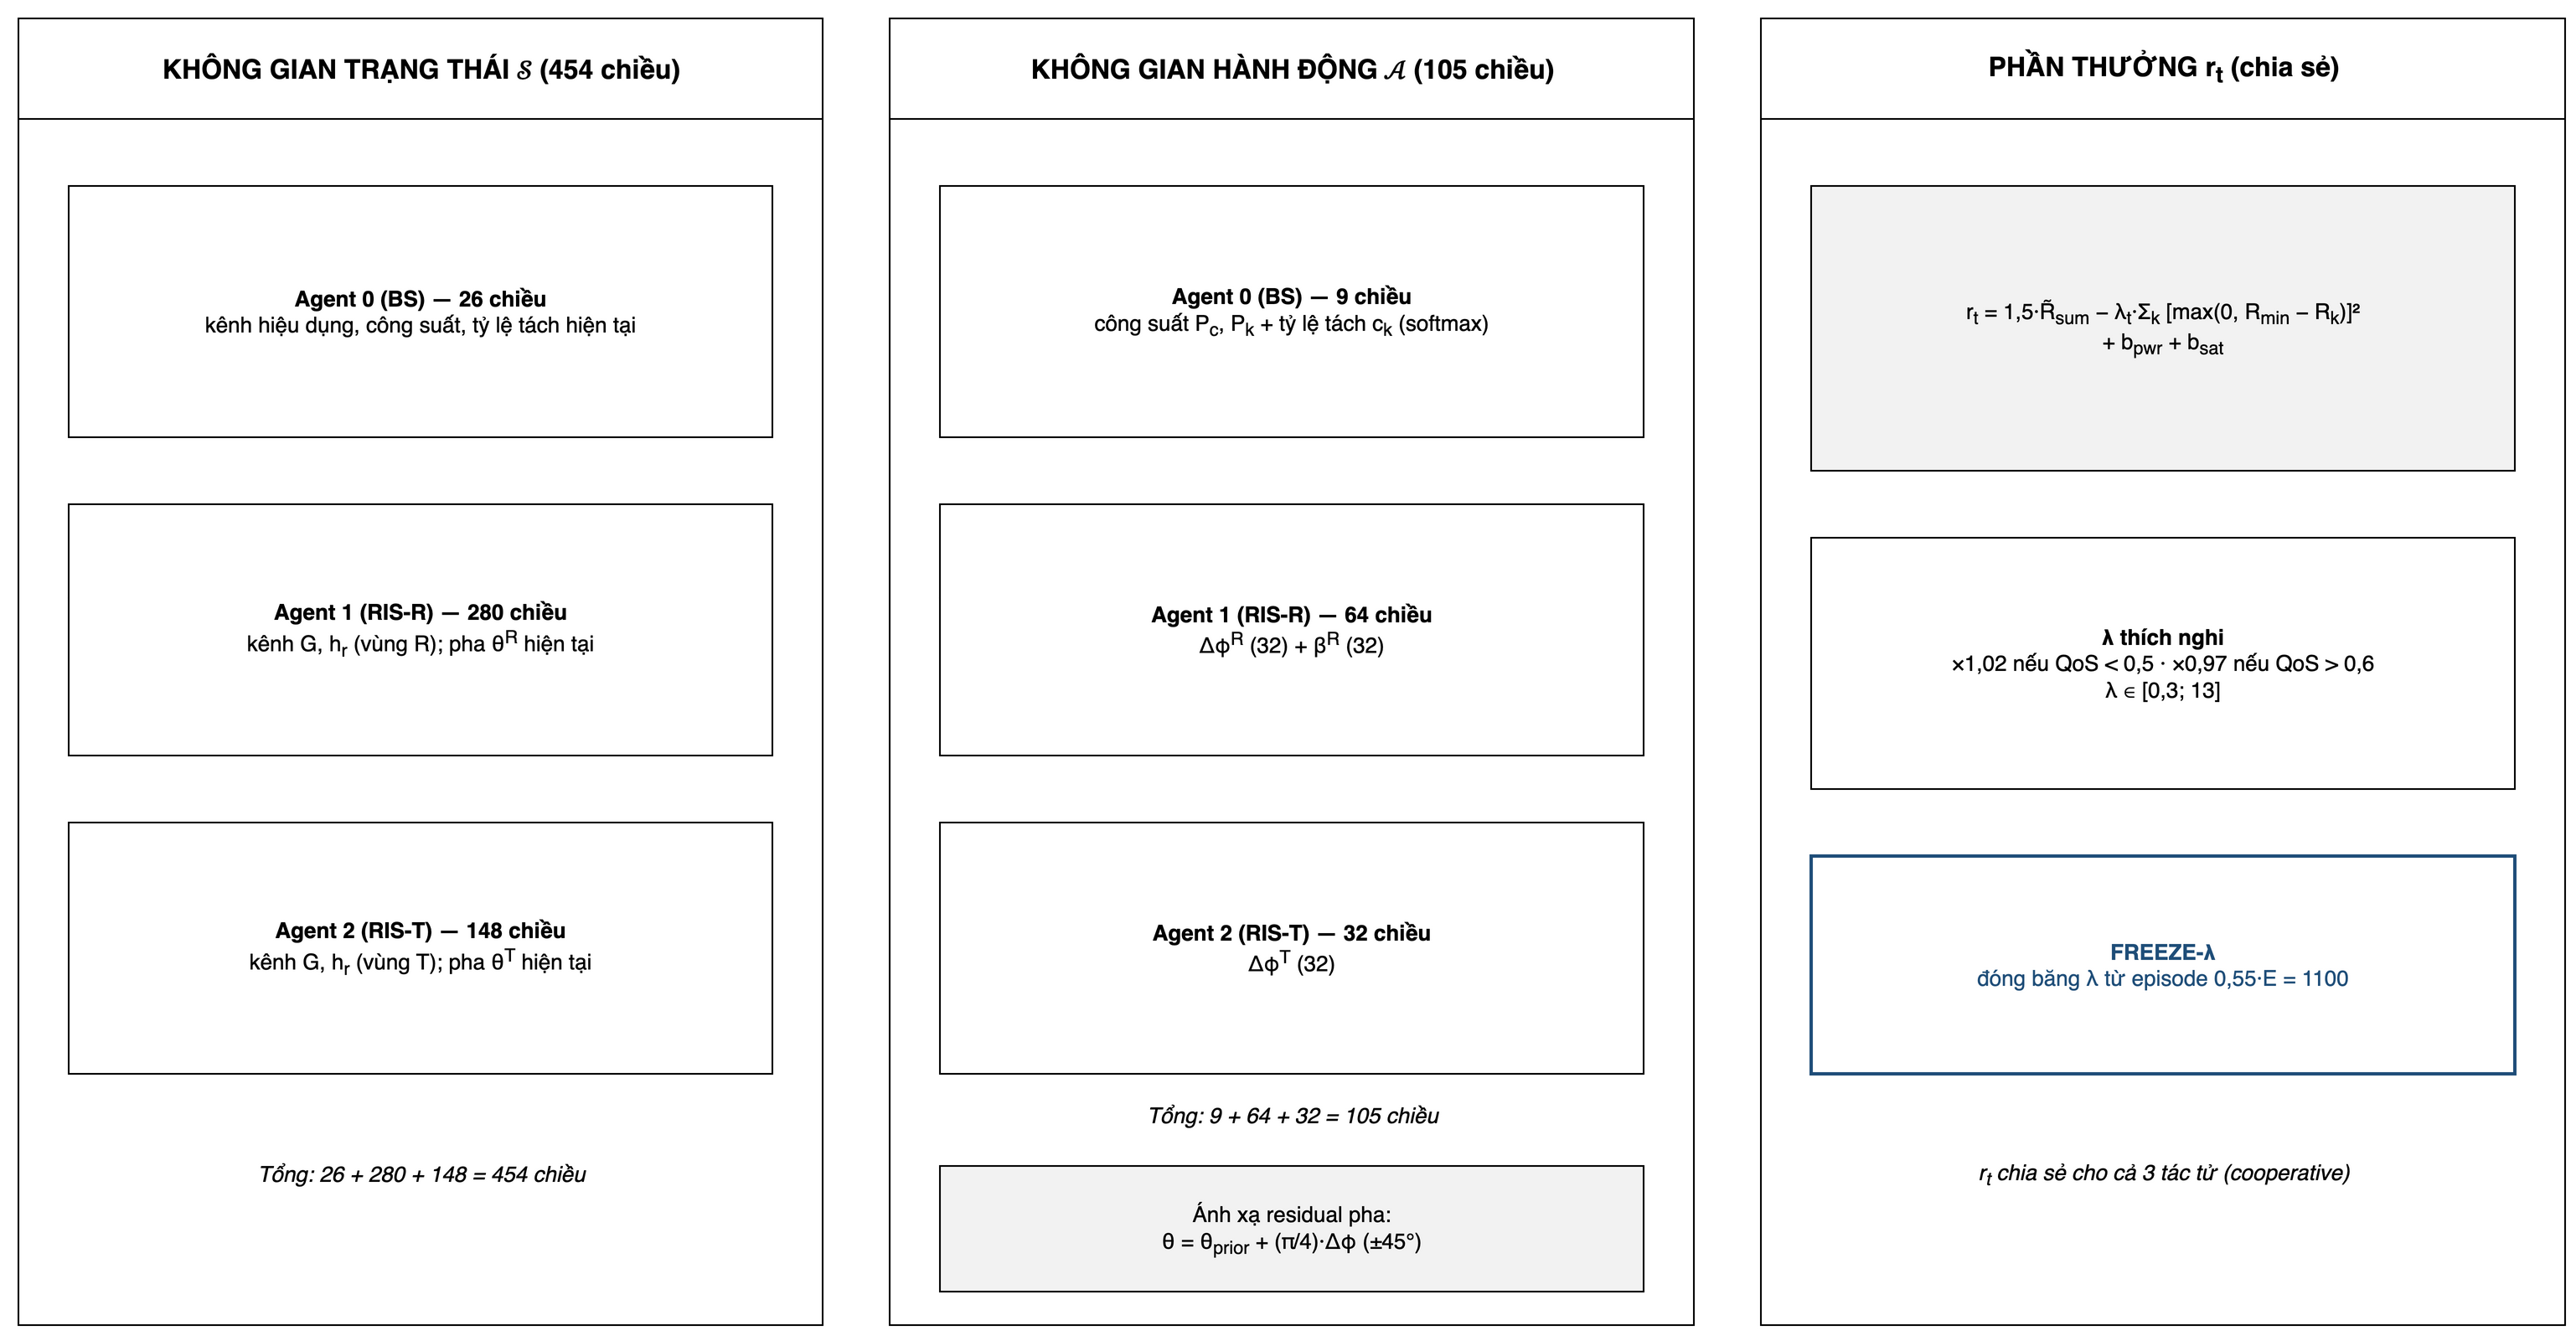
\includegraphics[width=0.96\linewidth]{figures/h2_5_mdp_anh_xa.png}
  \caption{Ánh xạ bài toán P0 sang MDP: không gian trạng thái 550 chiều
  (tổng quan sát cục bộ ba tác tử), không gian hành động 105 chiều,
  hàm phần thưởng Lagrangian surrogate với cập nhật đối ngẫu per-user.}
  \label{fig:h2_5}
\end{figure}

\subsection{Không gian trạng thái}

Trạng thái tổng thể $s_t$ là phép hợp các quan sát cục bộ của ba tác tử
$s_t = (o_{0,t}, o_{1,t}, o_{2,t})$, với tổng số chiều
$26 + 344 + 180 = 550$ (cấu hình chuẩn $K=4$, $K_R=3$, $N=32$). Mỗi quan
sát cục bộ bắt đầu bằng khối chung 18 chiều: phần thực và phần ảo của
kênh hiệu dụng $h_{\text{eff},k}$ (8), vector trọng số công suất softmax
ở bước trước (5), tỷ lệ tách ở bước trước (4) và phần thưởng bước trước
(1). Cụ thể:

\textbf{Tác tử BS (Agent 0, $o_0 \in \R^{26}$):} khối chung (18) cùng
phần thực/ảo của các kênh trực tiếp $h_{d,k}$ cho cả 4 UE (8).

\textbf{Tác tử STAR-RIS Reflection (Agent 1, $o_1 \in \R^{344}$):} khối
chung (18); phần thực/ảo của $h_{d,k}$ vùng R (6); của $\mathbf{G}$ (64);
của $\mathbf{h}_{r,k}^R$ với $k \in \{1,2,3\}$ (192); và trạng thái
STAR-RIS đang áp dụng: biên độ $\beta_n^R$ (32) cùng pha phản xạ hiện
hành $\phi_n^R$ (32).

\textbf{Tác tử STAR-RIS Transmission (Agent 2, $o_2 \in \R^{180}$):} khối
chung (18); phần thực/ảo của $h_{d,4}$ (2); của $\mathbf{G}$ (64); của
$\mathbf{h}_{r,4}^T$ (64); và 32 pha truyền qua hiện hành $\phi_n^T$.

Thành phần trạng thái STAR-RIS hiện hành là cần thiết cho tính Markov
của bài toán: chi phí tái cấu hình ở bước sau phụ thuộc cấu hình đang
áp dụng, nên cấu hình đó phải xuất hiện trong quan sát.

\subsection{Không gian hành động}

Tổng số chiều hành động là $9 + 64 + 32 = 105$:

\textbf{Tác tử BS (9 chiều):} 5 đại lượng cho công suất $\{P_c, P_1, \ldots,
P_K\}$ (qua softmax thành tỷ lệ rồi nhân với $P_{\max}$) và 4 đại lượng
cho tỷ lệ tách $\{c_1, \ldots, c_K\}$ (qua softmax để đảm bảo
$\sum c_k = 1$).

\textbf{Tác tử RIS-R (64 chiều), theo đúng thứ tự trong cài đặt:} 32 đại
lượng biên độ phản xạ $\{\beta_n^R\}_{n=1}^{N}$ (ánh xạ tuyến tính từ
$[-1,1]$ về $[0,1]$) đứng \emph{trước}, tiếp theo là 32 đại lượng phần dư
pha phản xạ $\{\Delta\phi_n^R\}_{n=1}^{N}$.

\textbf{Tác tử RIS-T (32 chiều):} 32 đại lượng phần dư pha truyền qua
$\{\Delta\phi_n^T\}_{n=1}^{N}$.

Tham số hóa pha kiểu residual (Chương 3 sẽ trình bày chi tiết):
\begin{equation}
\theta_n^X \;=\; \theta_n^{\text{prior},X} + \frac{\pi}{4}\,\Delta\phi_n^X,
\quad X \in \{R, T\},
\label{eq:residual_phase}
\end{equation}
giúp giảm khó khăn khám phá và tăng tốc hội tụ.

\subsection{Hàm phần thưởng: Lagrangian surrogate của P0}
\label{sec:reward_surrogate}

Ràng buộc QoS (C4) trong P0 là ràng buộc cứng. Trong khuôn khổ DRL, Luận
văn giải một bài toán \emph{surrogate} dạng phạt/Lagrangian của P0: ràng
buộc cứng được thay bằng ràng buộc kỳ vọng
$\mathbb{E}[c_k] \leq 0$ với hàm ràng buộc có dấu
$c_k = R_{\min} - R_k$ (tương đương $\mathbb{E}[R_k] \geq R_{\min}$).
Cách tiếp cận này \emph{không} bảo đảm QoS tại từng bước cho từng người
dùng; nó tối ưu điểm cân bằng throughput--QoS. Hàm phần thưởng:
\begin{equation}
\boxed{
r_t \;=\; \alpha\,\tilde R_{\text{sum}}
       \;-\; \sum_{k=1}^{K} \lambda_k\, c_{k,t}
       \;-\; \frac{w}{2} \sum_{k=1}^{K} \big[\max(0,\, c_{k,t})\big]^2
       \;-\; \eta_{\phi} C^{\phi}_t - \eta_{P} C^{P}_t - \eta_{\beta} C^{\beta}_t
}
\label{eq:reward}
\end{equation}
trong đó:
\begin{itemize}[leftmargin=*]
\item $\tilde R_{\text{sum}} = R_{\text{sum}}/R_{\text{ref}}$ là tổng tốc
độ chuẩn hóa theo tham chiếu $R_{\text{ref}}$ (tham số cấu hình
\texttt{reward\_rate\_reference}, giá trị $20$ b/s/Hz cho $K=4$);
$\alpha=1{,}5$;
\item $\lambda_k \geq 0$ là biến đối ngẫu riêng của từng người dùng, được
cập nhật bằng gradient đối ngẫu có phép chiếu trên trung bình episode
của chính $c_k$ (chi tiết ở Chương 3); số hạng bậc nhất dùng $c_k$
\emph{có dấu} như trong Lagrangian chuẩn;
\item $w$ là trọng số phạt bậc hai tăng cường (augmented penalty,
\texttt{augmented\_penalty\_weight}), chỉ tác dụng lên phần vi phạm
$\max(0, c_k)$;
\item $C^{\phi}_t, C^{P}_t, C^{\beta}_t$ là chi phí tái cấu hình pha,
công suất và biên độ so với hành động đã áp ở bước trước (chuẩn hóa
theo số chiều; bằng $0$ tại $t=0$), với các trọng số
$\eta_{\phi}, \eta_{P}, \eta_{\beta}$.
\end{itemize}
Hai chỉ số QoS được báo cáo tách bạch trong toàn bộ Luận văn:
\begin{align}
\text{user\_qos\_fraction} &= \frac{1}{K}\sum_{k=1}^{K}
\mathbf{1}\!\left[R_k \geq R_{\min}\right]
\quad\text{(tỷ lệ người dùng đạt QoS)},
\label{eq:user_qos_fraction}\\
\text{all\_users\_qos} &= \mathbf{1}\!\left[\min_k R_k \geq R_{\min}\right]
\quad\text{(tất cả người dùng đồng thời đạt QoS)}.
\label{eq:all_users_qos}
\end{align}
Đây là hai đại lượng khác nhau; mỗi bảng/hình đều ghi rõ metric nào
được dùng.

\subsection{Phân rã ba tác tử}

Hình \ref{fig:h2_6} biểu diễn phân rã ba tác tử chuyên dụng với chi tiết
các kích thước quan sát/hành động và kiến trúc Critic tập trung. Chi tiết
kiến trúc mạng và quy trình huấn luyện sẽ được trình bày trong Chương 3.

\begin{figure}[t]
  \centering
  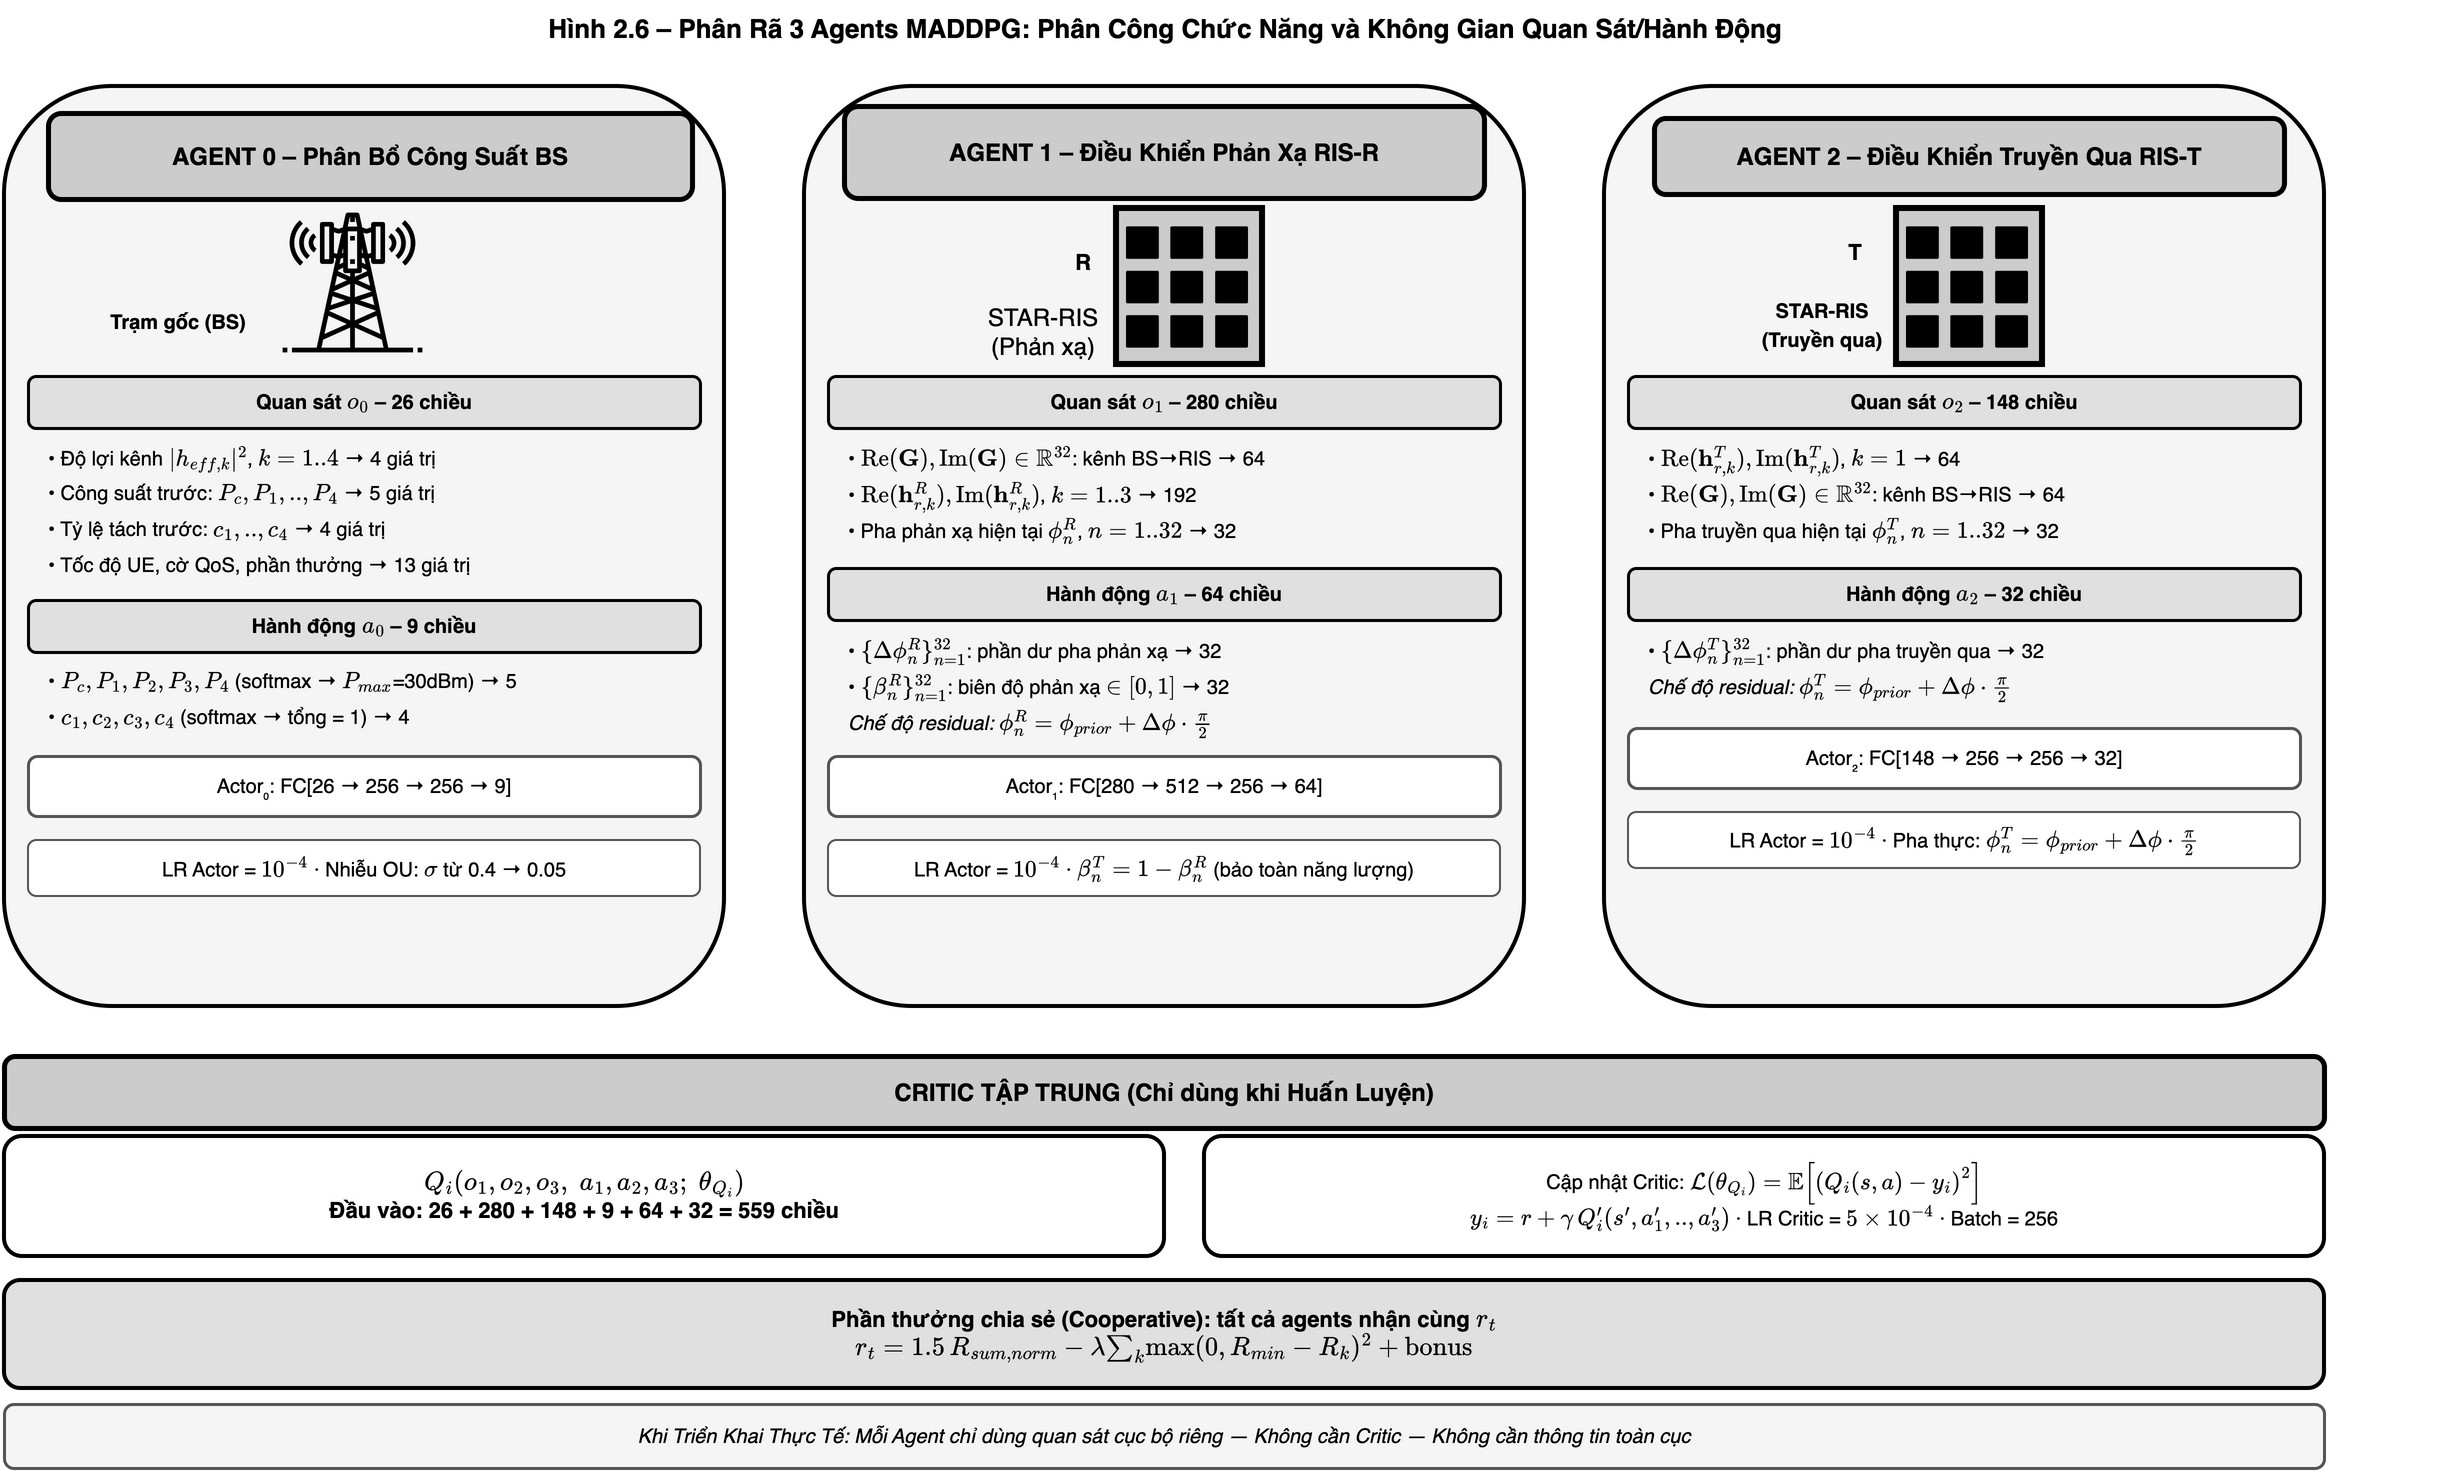
\includegraphics[width=0.96\linewidth]{figures/h2_6_3agents.png}
  \caption{Phân rã ba tác tử chuyên dụng: BS Power Agent ($26 \to 9$),
  RIS-R Agent ($344 \to 64$), RIS-T Agent ($180 \to 32$), và Critic tập
  trung với đầu vào $550 + 105 = 655$ chiều.}
  \label{fig:h2_6}
\end{figure}

% -----------------------------------------------------------------------------
\section{Tổng quan luồng hoạt động hệ thống}
\label{sec:overall_workflow}

Để định vị rõ ràng vai trò của khuôn khổ MADDPG đề xuất trong toàn bộ
hệ thống, Hình \ref{fig:overall_workflow} biểu diễn sơ đồ tổng quan
luồng hoạt động từ đầu cuối, gồm hai lớp được phân tách trực quan: lớp
vật lý (Physical Transmission Layer) chứa các khối truyền-nhận và lớp
điều khiển (MADDPG Controller) chứa các tác tử học.

\begin{figure}[t]
  \centering
  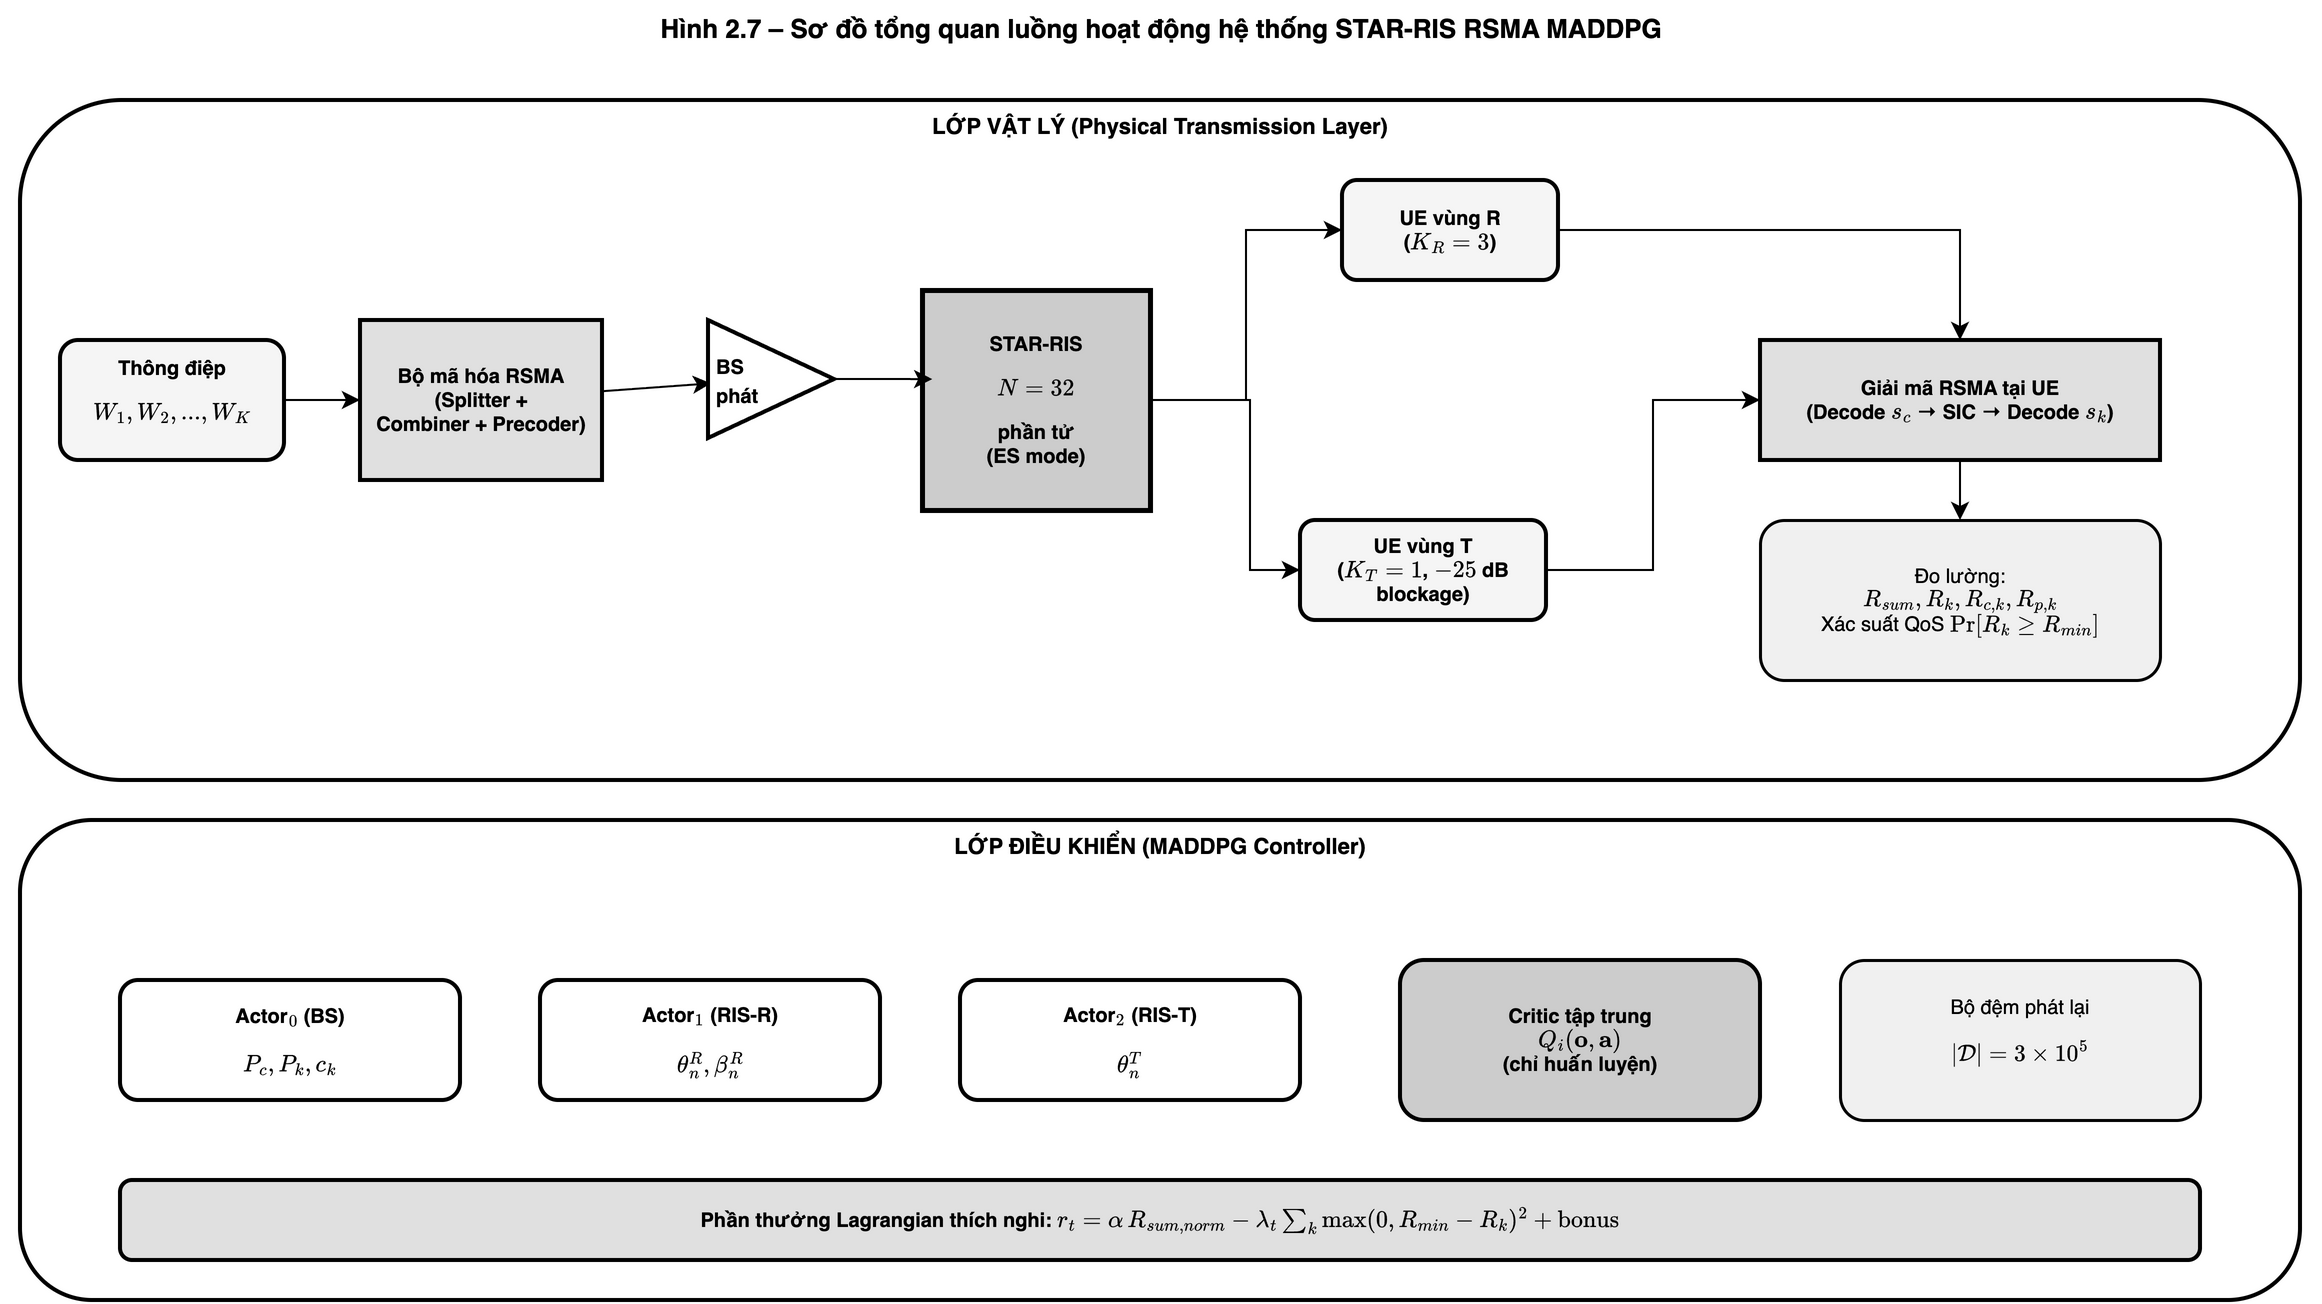
\includegraphics[width=0.98\linewidth]{figures/h2_7_overall_workflow.png}
  \caption{Sơ đồ tổng quan luồng hoạt động hệ thống STAR-RIS RSMA
  MADDPG. Lớp vật lý gồm bộ mã hóa RSMA, BS, STAR-RIS, các UE và các
  khối SIC, giải mã. Lớp điều khiển gồm ba tác tử Actor và Critic tập
  trung (chỉ dùng khi huấn luyện), được điều khiển bởi phần thưởng
  Lagrangian thích nghi.}
  \label{fig:overall_workflow}
\end{figure}

Luồng hoạt động end-to-end diễn ra như sau. Tại BS, thông điệp gốc
$\{W_k\}_{k=1}^K$ được bộ mã hóa RSMA tách thành luồng chung $s_c$ và
các luồng riêng $s_k$, sau đó kết hợp thành tín hiệu phát $x$ theo
\eqref{eq:rsma_signal}. Tín hiệu này được phát qua kênh trực tiếp
$h_{d,k}$ và đồng thời được điều hướng bởi STAR-RIS với hai ma trận
$\boldsymbol{\Phi}_R$ và $\boldsymbol{\Phi}_T$ tác động lên các vùng
phản xạ và truyền qua. Tại mỗi UE, quá trình giải mã RSMA gồm hai bước
nối tiếp: giải mã luồng chung, áp dụng SIC, sau đó giải mã luồng riêng.
Sum-rate và mức đáp ứng QoS đo được tại các UE được sử dụng làm tín
hiệu phản hồi (feedback) để tính phần thưởng $r_t$, từ đó cập nhật các
mạng Actor và Critic. Trong khi huấn luyện, Critic tập trung sử dụng
toàn bộ quan sát và hành động ghép $(\mathbf{o}, \mathbf{a})$ thông
qua các mẫu trong bộ đệm phát lại $\mathcal{D}$. Khi triển khai thực
tế, Critic được bỏ đi, chỉ ba Actor được giữ lại để sinh hành động
$\{a_{i,t}\}_{i=0,1,2}$ một cách phi tập trung dựa trên quan sát cục
bộ $o_{i,t}$.

% -----------------------------------------------------------------------------
\section*{Kết luận chương}
\addcontentsline{toc}{section}{Kết luận chương}

Chương 2 đã xây dựng đầy đủ mô hình hệ thống STAR-RIS hỗ trợ RSMA với
các thành phần BS-RIS-UE, mô hình kênh truyền (suy hao log-distance,
pha-đinh Rayleigh, chướng ngại $-25$~dB cho vùng T), và mô hình tín hiệu
RSMA với SINR và tốc độ. Bài toán tối ưu phân bổ tài nguyên P0
\eqref{eq:P0} được phát biểu với hàm mục tiêu max $R_{\text{sum}}$ và sáu
nhóm ràng buộc, đặc biệt bổ sung ràng buộc QoS trên từng người dùng.
Sau đó bài toán được ánh xạ sang MDP với ba tác tử chuyên dụng, không gian
trạng thái 550 chiều, không gian hành động 105 chiều và hàm phần thưởng
Lagrangian thích nghi. Chương 3 sẽ trình bày thiết kế chi tiết của khuôn
khổ MADDPG để giải MDP này.
